\tolerance=10000
\documentclass[conference]{IEEEtran}
\usepackage{xcolor}
\usepackage{mathtools}
\usepackage{enumerate}
\usepackage{multirow}
\usepackage{hyperref}
\usepackage{amssymb}
\usepackage{amsmath}
\usepackage{eqnarray}
\usepackage{booktabs}
\usepackage{array}
\usepackage[]{algorithm}
\usepackage{clrscode3e}
\usepackage[pdftex]{graphicx}

\definecolor{zblack}{HTML}{000000}
\definecolor{zblue}{HTML}{0072BD}
\definecolor{zred}{HTML}{D85319}
\definecolor{zyellow}{HTML}{BC9020}
\definecolor{zpurple}{HTML}{7E2F8E}
\definecolor{zgreen}{HTML}{77AC30}

%\usepackage{etoolbox}
%\AtBeginEnvironment{algorithmic}{\small}
%\usepackage{subfig}
% tricks for saving space
\usepackage[font={small}]{caption,subfig}  % small fonts in captions
\setlength{\abovecaptionskip}{1ex}
\setlength{\belowcaptionskip}{1ex}
\setlength{\floatsep}{1ex}
\setlength{\textfloatsep}{1ex}

\DeclarePairedDelimiter{\ceil}{\lceil}{\rceil}
\DeclarePairedDelimiter{\floor}{\lfloor}{\rfloor}
\DeclarePairedDelimiter{\angled}{\langle}{\rangle}

\begin{document}

%%%%%%%%%%%%%%%%%%%%%%%%%%%%%%%%%%%%%%%%%%%%%%%%%%%%%%%%%%%%%%%%%%%%%%%
%%%%%%%%%%%%%%%%%%%%%%%%%%%%%%%%%%%%%%%%%%%%%%%%%%%%%%%%%%%%%%%%%%%%%%%
%%
%% TITLE
%%
%%%%%%%%%%%%%%%%%%%%%%%%%%%%%%%%%%%%%%%%%%%%%%%%%%%%%%%%%%%%%%%%%%%%%%%
%%%%%%%%%%%%%%%%%%%%%%%%%%%%%%%%%%%%%%%%%%%%%%%%%%%%%%%%%%%%%%%%%%%%%%%

\title{ZNN\emph{i} -- Maximizing the Inference Throughput of 3D
  Convolutional Networks on Multi-Core CPUs and GPUs}

\author{\IEEEauthorblockN{Aleksandar Zlateski\IEEEauthorrefmark{1},
    Kisuk Lee\IEEEauthorrefmark{2}}
  \IEEEauthorblockA{\IEEEauthorrefmark{1}Electrical Engineering and
    Computer Science Dept.\\ \IEEEauthorrefmark{2}Brain and
    Cognitive Sciences Dept.\\ Massachusetts Institute of
    Technology\\ Cambridge, MA 02139 USA\\ \IEEEauthorrefmark{1}{\tt
      zlateski@mit.edu}, \IEEEauthorrefmark{2}{\tt kisuklee@mit.edu}}
  \and \IEEEauthorblockN{H. Sebastian Seung}
  \IEEEauthorblockA{Princeton Neuroscience Institute\\ and Computer
    Science Dept.\\ Princeton University\\ Princeton, NJ 08540
    USA\\ {\tt sseung@princeton.edu} }}


\maketitle
%\IEEEpeerreviewmaketitle
%\thispagestyle{empty}

%%%%%%%%%%%%%%%%%%%%%%%%%%%%%%%%%%%%%%%%%%%%%%%%%%%%%%%%%%%%%%%%%%%%%%%
%%%%%%%%%%%%%%%%%%%%%%%%%%%%%%%%%%%%%%%%%%%%%%%%%%%%%%%%%%%%%%%%%%%%%%%
%%
%% ABSTRACT
%%
%%%%%%%%%%%%%%%%%%%%%%%%%%%%%%%%%%%%%%%%%%%%%%%%%%%%%%%%%%%%%%%%%%%%%%%
%%%%%%%%%%%%%%%%%%%%%%%%%%%%%%%%%%%%%%%%%%%%%%%%%%%%%%%%%%%%%%%%%%%%%%%


\begin{abstract}
Sliding window convolutional networks (ConvNets) have become a popular
approach to computer vision problems such as image segmentation, and
object detection and localization. Here we consider the
parallelization of inference, i.e., the application of a previously
trained ConvNet, with emphasis on 3D images.  Our goal is to maximize
throughput, defined as the number of output voxels computed per unit
time.  We propose CPU and GPU primitives for convolutional and pooling
layers, which are combined to create CPU, GPU, and CPU-GPU inference
algorithms.  The primitives include convolution based on highly
efficient padded and pruned FFTs. Our theoretical analyses and
empirical tests reveal a number of interesting findings.  For example,
adding host RAM can be a more efficient way of increasing throughput
than adding another GPU or more CPUs.  Furthermore, our CPU-GPU
algorithm can achieve greater throughput than the sum of CPU-only and
GPU-only throughputs.
\end{abstract}

%%%%%%%%%%%%%%%%%%%%%%%%%%%%%%%%%%%%%%%%%%%%%%%%%%%%%%%%%%%%%%%%%%%%%%%
%%%%%%%%%%%%%%%%%%%%%%%%%%%%%%%%%%%%%%%%%%%%%%%%%%%%%%%%%%%%%%%%%%%%%%%
%%
%% INTRODUCTION
%%
%%%%%%%%%%%%%%%%%%%%%%%%%%%%%%%%%%%%%%%%%%%%%%%%%%%%%%%%%%%%%%%%%%%%%%%
%%%%%%%%%%%%%%%%%%%%%%%%%%%%%%%%%%%%%%%%%%%%%%%%%%%%%%%%%%%%%%%%%%%%%%%

\section{Introduction}

% cuDNN is described here~\cite{chetlur2014cudnn}
%We do max fragment pooling as described here~\cite{giusti2013fast}.
%Except that we are limiting the sizes of our output patches to have
%each dimension equal to the cartesian product of all corresponding
%dimensions of all pooling windows in the network.

We care about throughput.

\section{Convolutional networks}

  Short ConvNet desc...

  Each layer of the ConvNet takes as an input $f$ 3D images and
  produces $f'$ 3D images.  The inputs to a layer are referred as
  input feature--maps and the outputs as output feature--maps.

\subsection{Convolutional layer}

  ....

  What it does

\subsection{Pooling layer}

  What it does

\subsection{What do we study here}

  We study only layered networks -- the input to each layer is either
  a network input or the output of some other layer.  Our primitives
  do not have that restriction, we just use them that way to analyze
  some networks.

  We study networks with only convolutional and pooling layers.
  Convolutional layers are computationally most expensive, while the
  pooling layers can be replaced with so called max--fragment--poling
  layers to compute more pixels by reusing the computation from the
  previous layers...

  We assume that the transfer function is rectify linear, can be
  anything.

  dwell more..

  \begin{figure}
    \begin{center}
      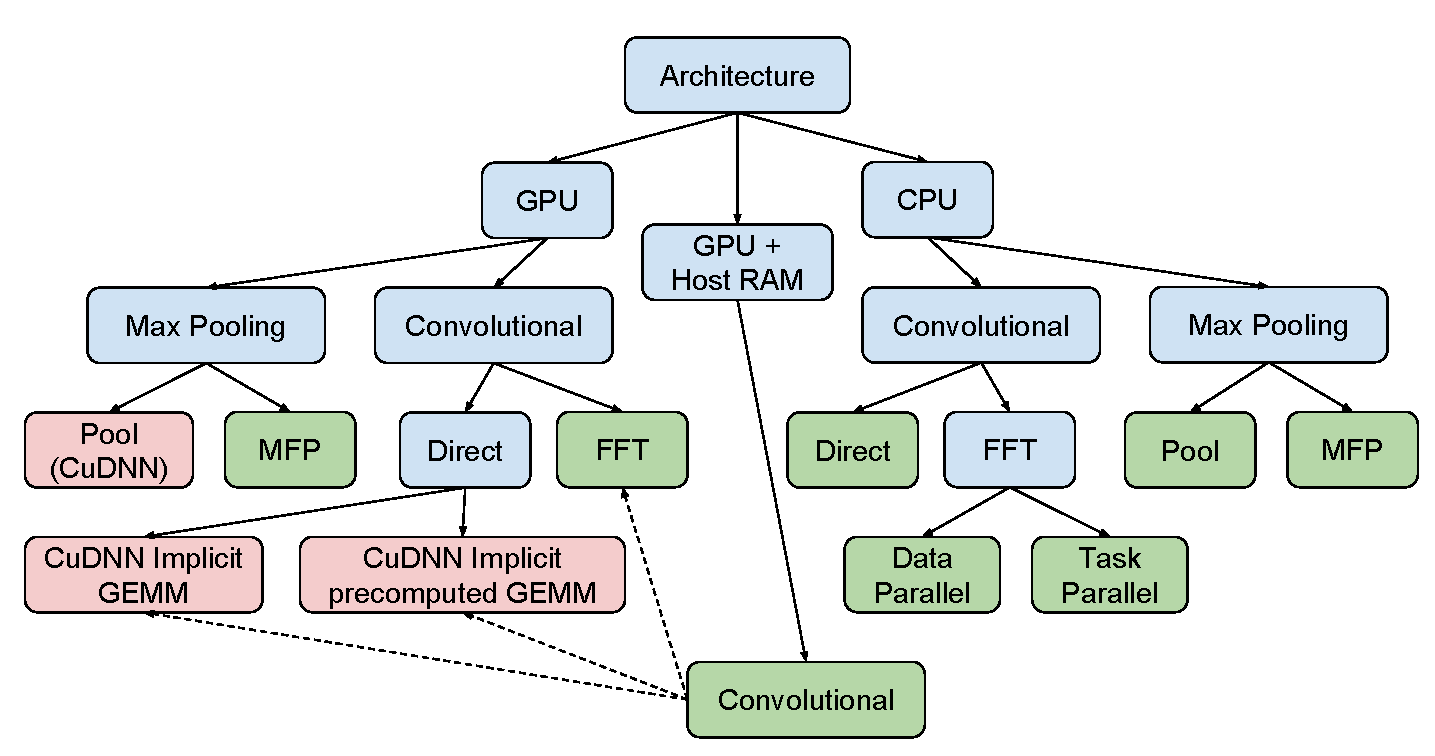
\includegraphics[width=0.99\columnwidth]{fig/alllayersram.pdf}
    \end{center}
    \caption{Diagram of all layers primitives.  The red primitives are
      wrappers primitives provided by CuDNN.  The green primitives are
      the novel primitives introduced in this paper.}
    \label{fig:layers}
  \end{figure}

\subsection{Contributions and novelty}

  - Introduction of new primitives for the CPU and GPU (list the novel ones)
     a) based on previously mentioned as tedious Padded Pruned FFTs
  - Showing how to use them to maximize throughput
  - Novel GPU + Host primitive
  - Showing how to use it
  - CPU + GPU pipeline algorithm

\section{Sliding window max--pooling ConvNet}

  \label{sec:sliding-window}

  A max-pooling ConvNet in the context of visual object
  recognition~\cite{krizhevsky2012imagenet} is a special case of the
  definition given above.  No max-filterings are used.  The size of
  the input image (known as the ConvNet field of view) is such that
  the convolutions and max-poolings reduce the output image(s) to
  exactly one pixel/voxel.  There may be a single output representing
  whether or not the input image belongs to a given object class, or a
  set of $n$ outputs representing membership in one of $n$ object
  classes.

  If localization and detection are desired as well as recognition,
  one can slide a window over a large image, and apply the max-pooling
  ConvNet at each location of the window
  \cite{sermanet2013overfeat}. For an input image of size $n^3$ and a
  ConvNet field of view of size $v^3$, the output image is of size
  $(n-v+1)^3$.  The sliding window max-pooling ConvNet is also useful
  in the context of boundary detection and image
  segmentation~\cite{ciresan2012deep}.

  However, it is computationally wasteful to literally implement the
  computation in this way.  The computational complexity can be
  reduced by either increasing the input image size which will produce
  sparse outputs. (Explain the limitations etc..) Or by more advanced
  methods such as
  \emph{max-fragment-pooling}~\cite{giusti2013fast,masci2013fast}
  where the pooling layers produce multiple output images, each of
  which is independently processed by all the subsequent layers.
  Another approach that produces equivalent results by using
  \emph{max-filtering} instead of max--pooling and increasing the
  sparsity of all subsequent convolutions by a factor equal to the
  size of the max--filtering window~\cite{zlateski2015znn} (This
  approach has also been called
  \emph{skip-kernels}~\cite{sermanet2013overfeat}, \emph{filter
    rarefaction}~\cite{long2015fully}, and \emph{dilated
    convolutions}~\cite{yu2015multi}).

  Long at al.~\cite{long2015fully} shows that the two approaches
  essentially perform the same computation, the only difference is the
  way the intermediate results are stored.  The \emph{MFP} approach
  has a very slightly lower computational complexity when FFT--based
  convolution is used, but might be tricky to implement for an
  arbitrary input image size.

  Input image sizes can be restricted to the ones for which all
  \emph{MFP} layers of a given ConvNet produce fragments of the same
  size.  This can further lower the computational complexity when
  FFT--based implementations are used, and greatly simplifies the
  performances.  Limiting the inputs to a specific size also limits
  the outputs to a specific size, which might be undesirable
  limitation when training a ConvNet.  For maximizing the inference
  throughput this limitation has no effect, as the goal is to obtain
  the result of a ConvNet applied to a large 3D image, with the amount
  of pixels computed at the time being irrelevant.

\section{Network execution}

  In the computational sense, each layer of a ConvNet takes a 5
  dimensional tensor $I$ as an input and produces another 5
  dimensional tensor $I'$.  The input tensor is in the form
  $(S,f,x,y,z)$ and the output $(S',f',x',y',z')$.  $S$ is the
  mini--batch size -- how many sets of inputs are provided.  $f$ and
  $f'$ are the number of input/output feature--maps of the layer, and
  $(x,y,z)$ and $(x',y',z')$ is the size of each input/output 3D
  image.

  We'll refer to the size of $I$ and $I'$ as input and output shape,
  respectively.  The relationship between the input shape and output
  shape will depend on the layer type, and kernel size in the case of
  a convolutional layer.

  In the simple case when only convolutional and max--pooling layers
  are present the mini--batch size of the input will be the same as
  the mini--batch size of the output ($S = S'$).

  When no \emph{max--fragment--pooling} (\emph{MFP}) layers are
  present

  The relationship between the two is shown in
  the columns 2 and 3 of
  Table~\ref{table:layers_complexity}\footnote{The table assumes
    isotropic 3D images.}.  Because all the dimensions of the input
  and output shape have to be integral, not every size of input and
  output shape is allowed.

  For the input shape $I = (S,f,x,y,z)$ with $S > 1$, the mini--batch
  size $S'$ of the output shape $I' = (S',f',x',y',z')$ will always be
  divisible by $S$.  The values $I'(\frac{S'}{S} i : \frac{S'}{S}
  (i+1),:,:,:,:)$ will only depend on $I(i,:,:,:,:)$.  This means that
  concatenating results of applying a layer on two inputs
  $I_1(S_1,f,x,y,z)$ and $I_2(S_2,f,x,y,z)$ will equal to the result
  of the concatenated input of size $(S_1+S_2,f,x,y,z)$.  This means
  that each layer can compute the result of the 5D input tensor $I$ by
  sequentially computing the result of each 4D sub--tensor.  However,
  having $S > 1$ can be computationally beneficial, especially when
  FFT--based convolution is used.

  We'll refer to the input shape to the first layer, as the input to
  the ConvNet, and the output of the last layer as the output of the
  ConvNet.

  \subsection{Maximizing inference throughput}

  [This text should maybe go somewhere above]

  ConvNet architecture represents an ordered set of layers, where each
  layer can be either convolutional or max--pooling\footnote{We focus
    on these two layer types because the convolutional is the
    computationally intensive one, and max--pooling allows for
    different implementations.}.  Furthermore, for each convolutional
  layer we are given the set of kernels, biases, and the transfer
  function, and for weach max--poling layer we are given the pooling
  window size.

  For a given ConvNet architecture, we can have different network
  implementations.  Each network implementation is composed of
  different implementation of the two layer types.  The different
  implementations of the convolutional layers produce the same result,
  but their speed depends on various things such as kernel sizes,
  number of input/output feature--maps and size of the 3D images.

  The choice between regular pooling and \emph{max--fragment--pooling}
  (\emph{MFP}) layer implementation determines what is the spatial
  distribution of the network when compared to the sliding window
  output???

  In order to maximize the throughput we provide algorithms fast and
  memory efficient primitives for direct and FFT--based convolutional
  layers, as well as max--pooling and max--fragment--poling.
  Figure~\ref{fig:layers} summarizes our basic primitives based on the
  architecture they run on, and layer type they implement.

  When executing a ConvNet on a single architecture (CPU--only or
  GPU--only), maximizing throughput can be represented by the
  following minimization problem:

  \begin{equation*}
    \begin{aligned}
      & \min_{\id{Shape}^{in}_1, \id{Impl}_i}
      & & \frac{\sum_{1 \le i \le L} \proc{Time}(\id{Impl}_i,\id{Shape}^{in}_i,\id{Shape}^{out}_i)}
      { \proc{Size}( \id{Shape}^{out}_L)} \\
      & \textrm{subject to} & &
      \id{Shape}^{in}_i = \id{Shape}^{out}_{i-1} \\
      & & &
      \proc{Type}(\id{Impl}_i) = \proc{Type}(Layer_i). \\
      & & &
      \proc{Out-Shape}(\id{Impl}_i,\id{Shape}^{in}_i) = \id{Shape}^{out}_i \\
      & & &
      \proc{Num-Inputs}(\id{Layer}_i) = \id{Shape}^{in}_i[2] \\
      & & &
      \id{Shape}^{out}_i[j] \in \mathbb{N}^+ \\
      & & &
      \proc{Memory}(\id{Impl}_i) \le M_{\max} \\
    \end{aligned}
  \end{equation*}

  We are trying to find an optimal input shape of the network
  $\id{Shape}^{in}_1$ and an implementation for each of the network
  layers $\id{Impl}_i$ such that the total time spent computing the
  output, divided by the number of elements of the output is
  minimized.  Note that for a fixed set of layer implementations
  $\id{Impl}_i$ and fixed input shape $\id{Shape}^{in}_1$, the
  network's output shape $\id{Shape}^{out}_L$ is uniquely determined.

  Naturally, the input shape of each layer has to be equal to the
  output shape of the previous layer, and each layer has to be of the
  same type defined by the network architecture.

  Furthermore, memory required for computation by each layer has to be
  smaller than some pre--defined constant (memory available to the CPU
  or GPU), depending on the architecture.

  As all input and output shapes have to be integral, choice of the
  output shape can limit the choice of max--pooling layer
  implementations and vice versa.

  There are multiple reasons why this minimization problem is hard.
  First, the actual time required for each layer implementation will
  depend on the architecture it is running on (number of cores for
  CPUs, or the GPU type).  Secondly, because of the memory constraint,
  a choice of one parameter can limit the available range of the other
  parameters.  For example, for large kernel sizes, increasing the
  input shape, can allow only use of slower direct convolution, as
  FFT--based convolution requires more memory.  Therefore, some
  exhaustive search has to be done.

  In general case, the exhaustive search can be performed by:

  \begin{enumerate}
    \item Loop over all possibilities for the pooling layers.  This
      will introduce constraints on the allowable input shapes.
    \item Loop over all allowed input shapes.
    \item Determine the best implementation for each convolutional
      layer.
  \end{enumerate}

  This is possible because for fixed choice of \emph{max--pooling} or
  \emph{MFP} of each pooling layer, and fixed input shape, the time
  and space required for each convolutional layer is uniquely
  determined.  We pick the fastest one that satisfies the memory
  constrain.

  Sometimes, for a given network architecture, the following two
  choices can be made by analytically analyzing the network:

  \begin{enumerate}
    \item The choice between \emph{max--pooling} and \emph{MFP} for
      the pooling layers.
    \item The choice of the input's shape mini--batch size $S$ -- the
      most significant dimension of the input shape.
  \end{enumerate}

\subsection{Max--pooling vs MFP}

  Giusti at al.~\cite{giusti2013fast} and Masci at
  al.~\cite{masci2013fast} show that \emph{MFP}
  layers will outperform the network using regular \emph{max--pooling}
  layers.  However, they limit the sizes of the output images of the
  \emph{max--pooling} networks to $1 \times 1 \times 1$, while
  allowing the \emph{max--fragment--polling} networks to have an
  arbitrary output shape.

  The minimal output shape of a given ConvNet is $(1,f'_L,1,1,1)$
  where $f'_L$ is the number of output feature--maps of the last layer
  of the network.  When the most significant dimension of the output
  shape equals to $1$, only \emph{max--pooling} layers can be used.
  In order to use \emph{max--fragment-pooling} layers, the output
  shape has to be of the form $(\alpha S_{\min},f'_L,x,y,z)$, where
  $S_{min} = \prod_{i \in \id{Pooling}} p^3_i$.  This is because each
  \emph{MFP} layer $i$ with a window size of
  $p_i^3$ creates $p_i^3$ fragments for each input.

  Consider a network in the form of 'CPCPCCCC' where 'C' represents a
  convolutional layer with the kernel size of

  It is well known (cite what?) that when the size of output images
  are increased, ConvNets require less operations per output pixel.

  As it turns out, when limited amount of RAM is available, a network
  using.


  \begin{figure}
    \centering
    \subfloat[]{\protect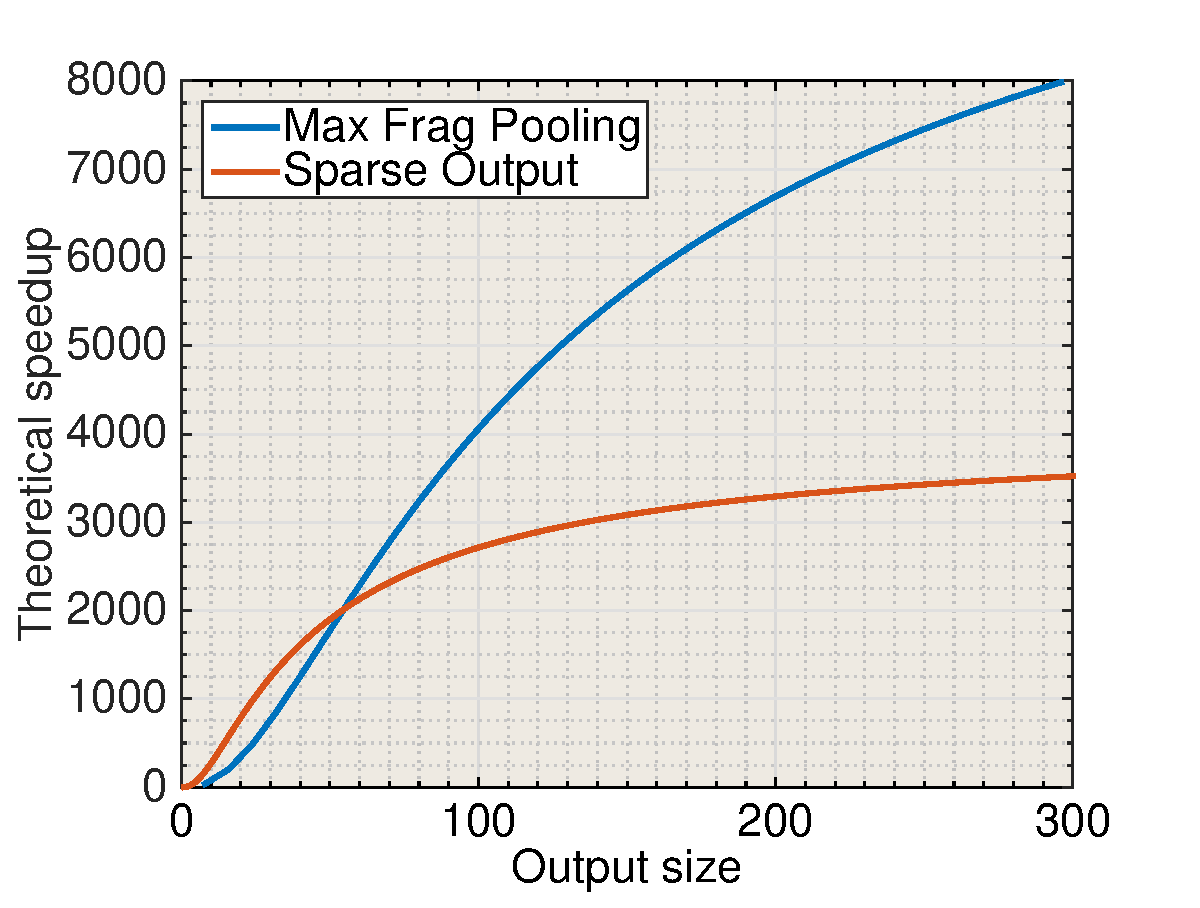
\includegraphics[width=0.24\textwidth]
      {fig/vssparsesize.eps}
      \label{fig:sparse_explanationa}
    }
    \subfloat[]{\protect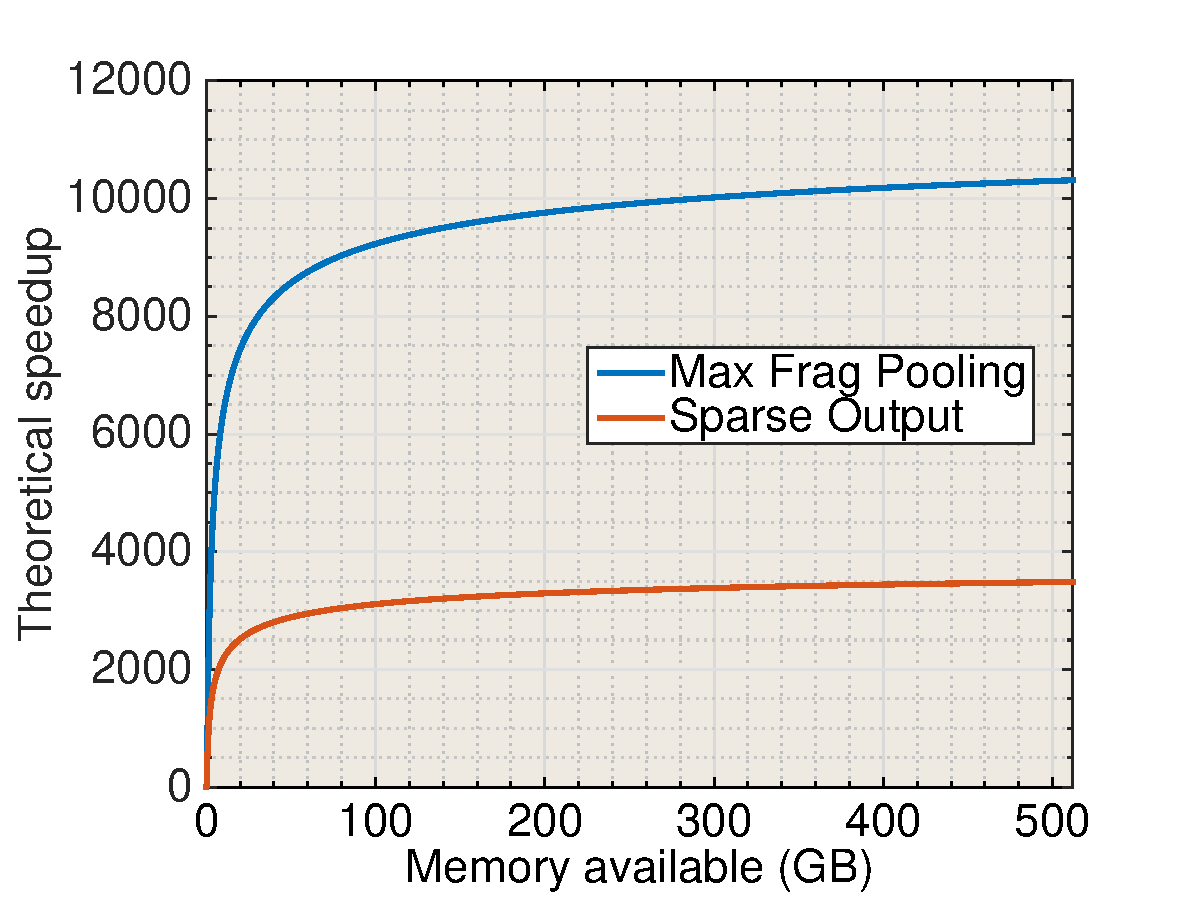
\includegraphics[width=0.24\textwidth]
      {fig/vssparsemem.eps}
      \label{fig:sparse_explanationb}
    }
    \caption{Comparison of the theoretical speedups of max--pooling
      and MFP ConvNets.}
    \label{fig:sparse_explanation}
  \end{figure}



  \begin{table*}[t]
    \centering
    \begin{tabular}{l|lll}
      \toprule
      Layer   & Input shape    & Output shape     & FLOPS \\
      \midrule
      Convolutional -- Direct &
      $S \times f \times n^3$ &
      $S \times f' \times [n-k]^3$ &
      $S \cdot f' \cdot f \cdot n^3 \cdot k^3$ \\
      Convolutional -- FFT--based &
      $S \times f \times n^3$ &
      $S \times f' \times [n-k]^3$ &
      $S \cdot 3Cn^3 \log n[f' + f] + 4Sf' \cdot f \cdot n^3 + f \cdot f' \cdot Cn \log n[k^2 + k \cdot n + n^2]$ \\
      Max Pooling &
      $S \times f \times n^3$ &
      $S \times f \times [n/p]^3$ &
      $S \cdot f \cdot n^3$ \\
      Max Fragment Pooling &
      $S \times f \times n^3$ &
      $[S \cdot p^3] \times f \times (n/p)^3$ &
      $S \cdot f \cdot n^3 \cdot p^3$ \\
      \bottomrule
    \end{tabular}
    \caption{Computational complexities.}
    \label{table:layers_complexity}
  \end{table*}

\section{FFT of padded image}
  The computational complexity of a ConvNet can be reduced by using
  FFT convolutions.  The advantages of such approach have been shown
  for 2D ConvNets running on
  GPUs~\cite{mathieu-iclr-14,vasilache2014fast}, and 3D ConvNets
  running on CPUs~\cite{zlateski2015znn}.

  In FFT convolution the kernel and the image are zero-padded to a
  common size.  Since the kernel is typically much smaller than the
  image, the padded kernel consists mostly of zeros.  If the FFT
  computation were implemented to ignore the zeros of the padded
  kernel, it would become much faster and use less memory.  We
  propose such an algorithm, and implement it for both the CPU and
  GPU. Our approach achieves an average of $5 \times$ speedup over the
  naive approach on the CPU and $10 \times$ speedup on the GPU.  It
  also greatly reduces the memory overhead compared to the approaches
  described in ~\cite{mathieu-iclr-14,vasilache2014fast}.

  The speedup is expected to be large for a ConvNet, which typically
  contains many more kernel FFTs than image FFTs.  The speedup is more
  modest for a single convolution, which requires one padded kernel
  FFT, one image FFT, and one inverse FFT.

  Our padded FFT algorithms are the foundation of our FFT--based
  convolutional layers, but understanding them is not necessary for
  understanding the latter part of the paper.

\subsection{Padded FFT algorithm}

  \begin{figure}
    \begin{center}
      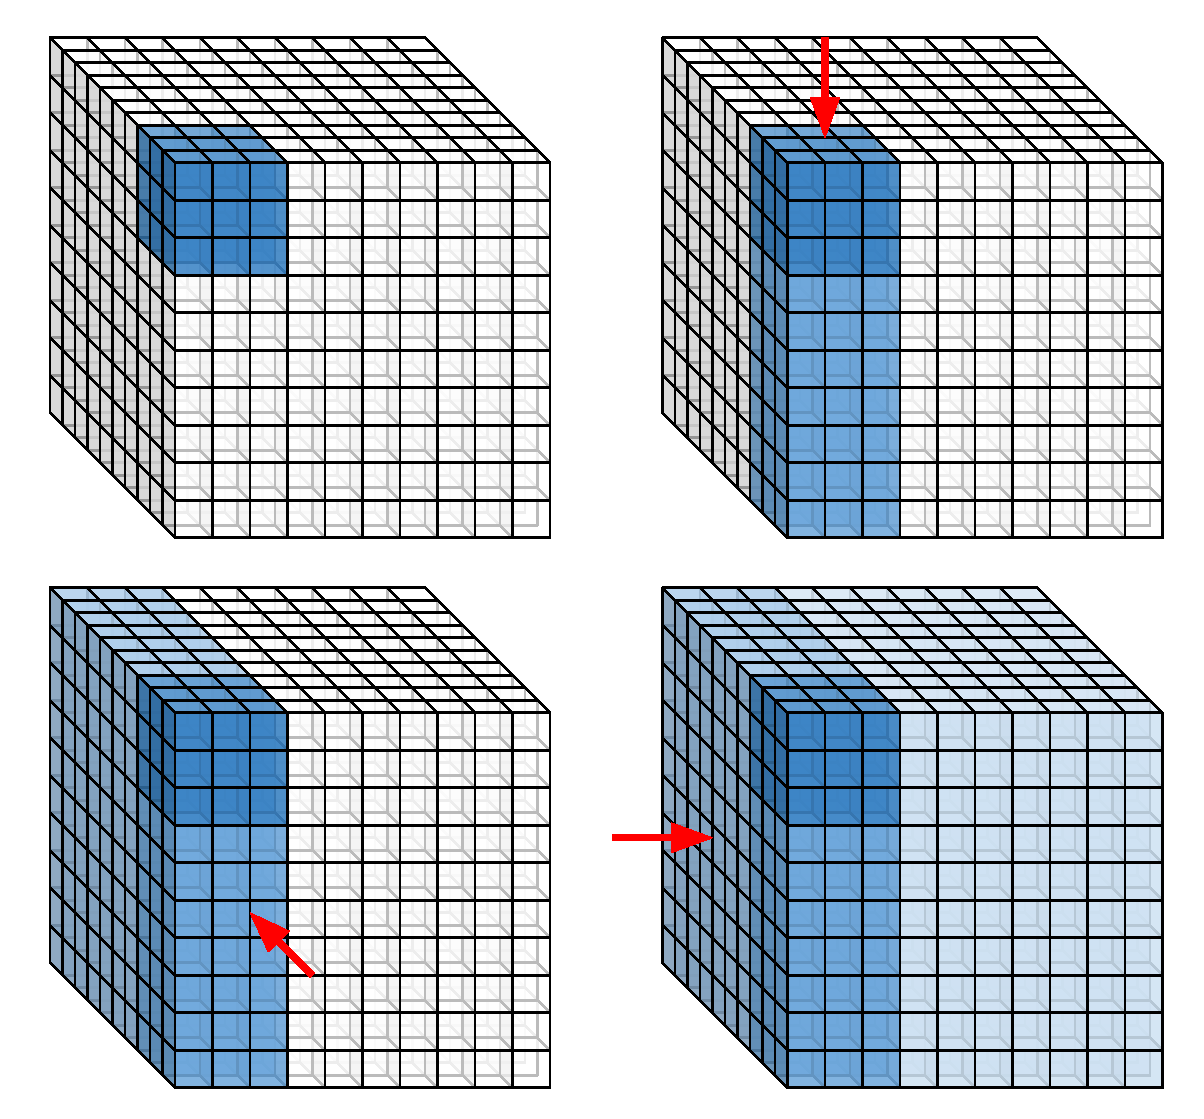
\includegraphics[width=0.55\columnwidth]{fig/pruned_ffts.pdf}
    \end{center}
    \caption{Pruned FFTs.}
    \label{fig:pruned_ffts}
  \end{figure}

  For 3D FFT--based convolution, the 3D images $x$ and $y$ are first
  zero-padded to the same size.  The inverse FFT of the point-wise
  product contains the result of the convolution.  The images $x$ and
  $y$ can be zero-padded to any size, as long as their size is equal.

  A 3D FFT is obtained by computing 1D FFTs along the three
  dimensions.  Some of these 1D FFTs are of an array with all elements
  equal to $0$.  These are unnecessary to compute as the FFT of
  a \emph{all zeros} signal is all zeros.

  We can reduce the amount of computation by computing only necessary
  1D transforms.  When computing the FFT of a trainable kernel of size
  $k^3$ zero padded to size of $n^3$, instead of naively computing
  $n^2$ 1D FFTs each dimension, which takes $C n^3 \log n^3$ we could
  first only do $k^2$ FFTs along one direction, then $k \times x$
  along then next, and finally $n^2$ along the last direction, as
  shown on Figure~\ref{fig:pruned_ffts}.  This approach reduces the
  computational cost from $C n^3 \log n^3$ to $C n\log n[k^2 + k \cdot
    n + n^2]$.  As most of the FFTs are performed on kernels, and as
  the kernel sizes are usually much smaller compared to the image
  sizes ($k \ll n$), we could reduce the computation cost by nearly two
  thirds.

  Our approach uses $3$rd party libraries to perform a batch of 1D
  FFTs.  Depending on the library implementation, the size to which we
  pad the 3D image can greatly influence the computational complexity.

  On the CPU we use either {\tt fftw} or {\tt Intel MKL}, and pad the
  images (and kernels) to sizes that can be written in the form of
  $2^a3^b5^c7^d11^e13^f$.  When {\tt Intel MKL} is used any such size
  is allowed, however, when {\tt fftw} is used we only allow sizes for
  which $e+f$ is either $0$ or $1$~\cite{frigo1999fftw,frigo1998fftw}.
  On the GPU we use cuFFT~\cite{nvidia2010cufft}, which has optimized
  algorithms only for sizes of the form $2^a3^b5^c7^d$.

  We proceed to propose an algorithm that computes the FFT (and
  inverse FFT) of an image of size $x \times y \times z$ zero-padded
  to the size of $x' \times y' \times z'$.

\subsection{CPU implementation}
  The $x \times y \times z$ image is zero-padded to $x' \times
  y \times z$.  This is easily implemented by doing a linear copy of
  the memory, and zero-padding the rest. We then perform $y \cdot z$
  1D real to complex FFT transforms along the $x$ direction.  The FFTs
  are performed out of place into a pre-allocated, and
  zero-initialized complex-valued $\floor{\frac{x'}{2}} + 1 \times
  y' \times z'$ image.  We then perform in-place 1D transforms along
  the $y$ direction, followed by the $z$ direction.

  The inverse FFT is computed by following the above steps in reverse
  order.  The 1D FFTs can either be done serially, or by $N$ workers
  in parallel (in a parallel for loop).

% say smth about memory requirement?

\subsection{GPU implementation}

\label{sec:gpu-fft-impl}

  Our GPU algorithm always performs FFTs on $b$ 3D images
  simultaneously, in order to achieve high utilization of the many
  GPU threads.

  A set of $b$ 3D images can be represented as a 4D tensor.  We need
  to perform 1D FFTs along the three least significant dimensions.
  Our algorithm computes the 3D FFTs as a series of tensor
  transforms~\footnote{This is known as a \texttt{permute} function in
    MATLAB} and 1D FFTs along the least significant dimension of the
  tensor.

  When computing the FFT transforms of $b$ 3D images each of size $x
  \times y \times z$ padded to $x' \times y' \times z'$, the size of
  the 4D input tensor $I$ is $b \times x \times y \times z$.  First,
  1D in--place real to complex 1D transforms along the $z$ direction
  are performed. We prepare the input by extending the 4D tensor along
  the $z$ direction to fit the result.  The transform will need to
  contain $z'' = z' / 2 + 1$ complex numbers, and we need twice as
  many reals.  A 4D tensor $I^1$ of size $b \times x \times y \times
  2z'')$ is first initialized to zero, and appropriate elements from
  the input are filled in (elements $I_{i,j,k,l}$ get mapped to
  $I^1_{i,j,k,l}$ while the rest of elements of $I^1$ are set to
  zero).

  A batch of $b$ in--place real to complex 1D transforms are then
  performed.  The result represents a 4D complex tensor
  $\widetilde{I}^1$ of size $b \times x \times y \times z''$.  Note
  that all the 1D transforms are done on contiguous memory chunks
  (along the least significant dimension).

  In the next step we perform in-place complex to complex transforms
  along the $y$ direction.  To do this the elements of
  $\widetilde{I}^1$ are permuted into another 4D tensor
  $\widetilde{I}^2$ of size $b \times x \times z'' \times y'$, such
  that the element $\widetilde{I}^1_{i,j,k,l}$ gets mapped to
  $\widetilde{I}^2_{i,j,l,k}$ and the rest of $\widetilde{I}^2$ is
  zero--filled.  We then perform in-place complex to complex
  transforms along the least significant dimension of
  $\widetilde{I}^2$.

  In the final step, we perform the transform along the $x$ direction.
  We permute $\widetilde{I}^2$ into a new 4D complex tensor
  $\widetilde{I}^3$ of size $b \times z'' \times y' \times x'$.  An
  element $\widetilde{I}^2_{i,j,k,l}$ is mapped to
  $\widetilde{I}^3_{i,k,l,j}$.  Complex to complex in-place transforms
  are performed along the least significant dimension of
  $\widetilde{I}^3$.

  As we only perform point-wise multiplications of transformed images,
  or take the inverse transforms of them, we can just keep the result
  in this representation -- not waste computation doing extra
  permuting.

  The inverse transform can be performed taking the same steps in
  reverse order.

  {\bf Implementation details} 4D tensor permuting requires a lot of
  indexing calculation, which can involve a lot expensive division and
  modulus operations.  Sometimes these operations are more expensive
  than the actual 1D FFT transforms performed.  We improve the
  performances by only using multiplications by a pre--computed magic
  numbers and shift operations as described in
  ~\cite{warren2013hacker}.  Image reshaping is easily implemented
  using the Thrust CUDA library~\cite{bell2011thrust}.

  We limit the large cuFFT memory overhead for computing batches of 1D
  transforms by splitting the batch computation into sub--batches of
  1D transforms.  We make sure that the sub--batch size is still large
  enough to utilize all the computational power, but limit the size so
  that we limit the memory overhead.  (Maybe mention that we have to
  keep the pointers to texture alignment?)

  The memory overhead of the algorithm is due to the fact that we do
  out-of-place permuting of the 4D tensor, and requires space for $b
  \cdot x \cdot y' \cdot z''$ complex numbers.  This, however, will
  not increase the memory overhead of our algorithm for convolutional
  layers on the GPU, as it already needs a temporary tensor of size $b
  \cdot x' \cdot y' \cdot z''$ for other purposes, which we can use as
  the scratch space for computing the FFT transforms.

  Additional, relatively small, overhead comes from the memory
  required by cuFFT to perform a batch of 1D transforms.  By dividing
  the batch into sub--batches we essentially limit this overhead to a
  pre--defined constant amount of memory.

\section{Convolutional layers}
  The input to a convolutional layer is a tuple of $f$ images, and the
  output a tuple of $f'$ images.  We want to process a batch of $S$
  inputs to yield a batch of $S$ outputs, via
  $$O_{s,j} = \sum_{i=1}^f w_{ji}\ast I_{s,i}$$ for $1 \le s \le S$
  and $1 \le j \le f'$.  Here $I_{s,i}$ is the $i^{th}$ image of the
  $s^{th}$ input in the batch, and $O_{s,j}$ is the $j^{th}$ image of
  the $s^{th}$ output in the batch, and $w_{ji}$ is the kernel from
  the $i$th image in an input tuple to the $j$th image in an output
  tuple.

We will assume 3D images and kernels.  If $I_{s,i}$ has size $\vec{n}
= \angled{n_x, n_y, n_z}$ and $w_{ji}$ has size $\vec{k}
= \angled{k_x,k_y,k_z}$, then we can regard $I$ as a 5D tensor of size
$S \times f \times n_x \times n_y \times n_z$, $w$ as a 5D tensor of size
$f' \times f \times k_x \times k_y \times k_z$, and $O$ as a 5D tensor of
size $S \times f' \times n_x' \times n_y' \times n_z'$, where
$\vec{n}' = \vec{n} - \vec{k} + \vec{1}$.

\subsection{CPU algorithms}

  We propose three parallel algorithms for the convolutional layer
  that are suited for multi-core CPUs.  The first algorithm performs
  direct convolution, whereas the other two use FFT based
  convolutions.

\subsubsection{Direct convolution algorithm}

  \begin{algorithm}
    {\small
      \begin{codebox}
        \Procname{$\proc{Convolutional-Forward-FFT-CPU1}(I,w,S,f,f',\vec{n},\vec{k})$}
        \li $\vec{n}' = \vec{n} - \vec{k} + \vec{1}$
        \li $O \gets \proc{5D-Real-Tensor}(S,f',n'_x,n'_y,n'_z)$
        \li \kw{parallel for} $i \gets 0 \To S-1$
        \li   \Do \kw{parallel for} $j \gets 0 \To f'-1$
        \li     \Do \For $k \gets 0 \To f-1$
        \li     \Do $O_{i,j} \gets O_{i,j} + \proc{Convolve}(I_{i,k},w_{j,k})$
        \End \End \End
        \li $\proc{Free-Memory}(I)$
        \li \Return $O$
      \end{codebox}
    }

    \caption{Multi-core algorithm for a convolutional layer using direct
      convolution.}
    \label{alg:cpu_direct}
  \end{algorithm}

  The algorithm using direct convolution is showin in the
  Algorithm~\ref{alg:cpu_direct}.  The computation is parallelized by
  two $\kw{parallel for}$ loops such that each output image of each
  minimbatch is computed in parallel on a different working thread.
  The $\kw{parallel for}$ loops are implemented using intel$^{\small
    \textregistered}$ thread building blocks such that the work is
  evenly divided over the available cores.

  For the direct convolution we provide two implementations.  The
  first is a naive convolution implementation, and the second one is
  using Intel$^{\small \textregistered}$ to perform convolutions.  MKL
  implementation is 2x faster on average, however it requires extra
  memory for a temporary image where a result of convolution is stored
  before accumulating it to the output image.  When $T$ cores are
  utilized, the algorithm yields a memory overhead of $T \times n_x'
  \times n_y' \times n_z'$.  The total amount of memory required for a
  layer is given in the Table~\ref{table:memory_requirements}.

  \begin{table}
    \centering
    \begin{tabular}{l >{$}l<{$}}
      \toprule
      CPU algorithm & \text{Memory required} \\
      \midrule
      Direct (naive) &
      S \cdot f \cdot n + S \cdot f' \cdot n'\\
      Direct (MKL) &
      S \cdot f \cdot n + S \cdot f' \cdot n' + T \cdot n' \\
      FFT algorithm 1 &
      \max
      \begin{cases}
        S \cdot f \cdot (n + \widetilde{n}) \\
        S \cdot f' \cdot n' + (S \cdot f + 1) \cdot \widetilde{n}
      \end{cases} \\
      FFT algorithm 2 &
      \max
      \begin{cases}
        S \cdot f \cdot (n + \widetilde{n}) \\
        S \cdot (f + f') \cdot \widetilde{n} + T \cdot \widetilde{n} \\
        S \cdot f' \cdot (n' + \widetilde{n})
      \end{cases} \\
      \bottomrule
      \toprule
      GPU algorithm & \text{Memory required} \\
      \midrule
      cuDNN (default) &
      S \cdot f \cdot n + S \cdot f' \cdot n' \\
      cuDNN (precomp) &
      2S \cdot f \cdot n + S \cdot f' \cdot n' \\
      FFT &
      C + \max
      \begin{cases}
        S \cdot f \cdot (n + \widetilde{n}) + f \cdot \widetilde{n} \\
        S \cdot (f + f') \cdot \widetilde{n} + 2f \cdot \widetilde{n} \\
        S \cdot f' \cdot (n' + \widetilde{n}) + f' \cdot \widetilde{n}
      \end{cases} \\
      \bottomrule
    \end{tabular}

    \caption{Memory required by different implementations.}
    \label{table:memory_requirements}
  \end{table}

\subsubsection{Data parallel FFT-based algorithm}

  The data parallel algorithm is given in the
  Algorithm~\ref{alg:cpu_fft_alg1}.  The computationally intensive
  operations in the algorithm are individually parallelized.  More
  specifically each FFT and inverse FFT transform is done in parallel
  as explained in the previous section.  The $\proc{Parallel-MAD}$
  function computes a series of multiply-add operations of complex
  numbers in parallel by dividing the range into roughly equal
  sub-ranges, each of which is executed on a single core.

  \begin{algorithm}
    {\small
      \begin{codebox}
        \Procname{$\proc{Convolutional-Forward-FFT-CPU1}(I,w,S,f,f',\vec{n},\vec{k})$}
        \li $\vec{n}' = \vec{n} - \vec{k} + \vec{1}$
        \li $\vec{\widetilde{n}} = \proc{FFT-Optimal-Size}(\vec{n})$
        \li $\widetilde{I} \gets \proc{5D-Complex-Tensor}(S,f,\floor{\widetilde{n}_x/2}+1,\widetilde{n}_y,\widetilde{n}_z)$
        \li \For $i \gets 0 \To S-1$
        \li   \Do \For $j \gets 0 \To f-1$
        \li     \Do $\widetilde{I}_{i,j} \gets \proc{Parallel-FFT}(I_{i,j})$
        \End \End
        \li $\proc{Free-Memory}(I)$
        \li $O \gets \proc{5D-Real-Tensor}(S,f',n'_x,n'_y,n'_z)$
        \li $\widetilde{O} \gets \proc{4D-Complex-Tensor}(S,\floor{\widetilde{n}_x/2}+1,\widetilde{n}_y,\widetilde{n}_z)$
        \li $\widetilde{w} \gets \proc{3D-Complex-Tensor}(\floor{\widetilde{n}_x/2}+1,\widetilde{n}_y,\widetilde{n}_z)$
        \li \For $i \gets 0 \To f'-1$
        \li   \Do \For $j \gets 0 \To f-1$
        \li     \Do $\widetilde{w} = \proc{Parallel-FFT}(w_{i,j})$
        \li         \For $k \gets 0 \To S-1$
        \li           \Do $\proc{Parallel-MAD}(\widetilde{I}_{k,j}, \widetilde{w}, \widetilde{O}_{k})$
        \End \End
        \li   \For $k \gets 0 \To S-1$
        \li      \Do $O_{k,i} \gets \proc{Parallel-Inverse-FFT}(\widetilde{O}_{k})$
        \End \End
        \li $\proc{Free-Memory}(\widetilde{I})$
        \li $\proc{Free-Memory}(\widetilde{O})$
        \li $\proc{Free-Memory}(\widetilde{w})$
        \li \Return $O$
      \end{codebox}
    }

    \caption{Multi-core algorithm for a convolutional layer}
    \label{alg:cpu_fft_alg1}
  \end{algorithm}

  The memory requirement of the algorithm equals to the maximal amount
  of memory required by the algorithm at any single point of time
  during the execution, and is given in
  Table~\ref{table:memory_requirements}.

\subsubsection{Task parallel FFT-based algorithm}

  \begin{figure}
    \begin{center}
      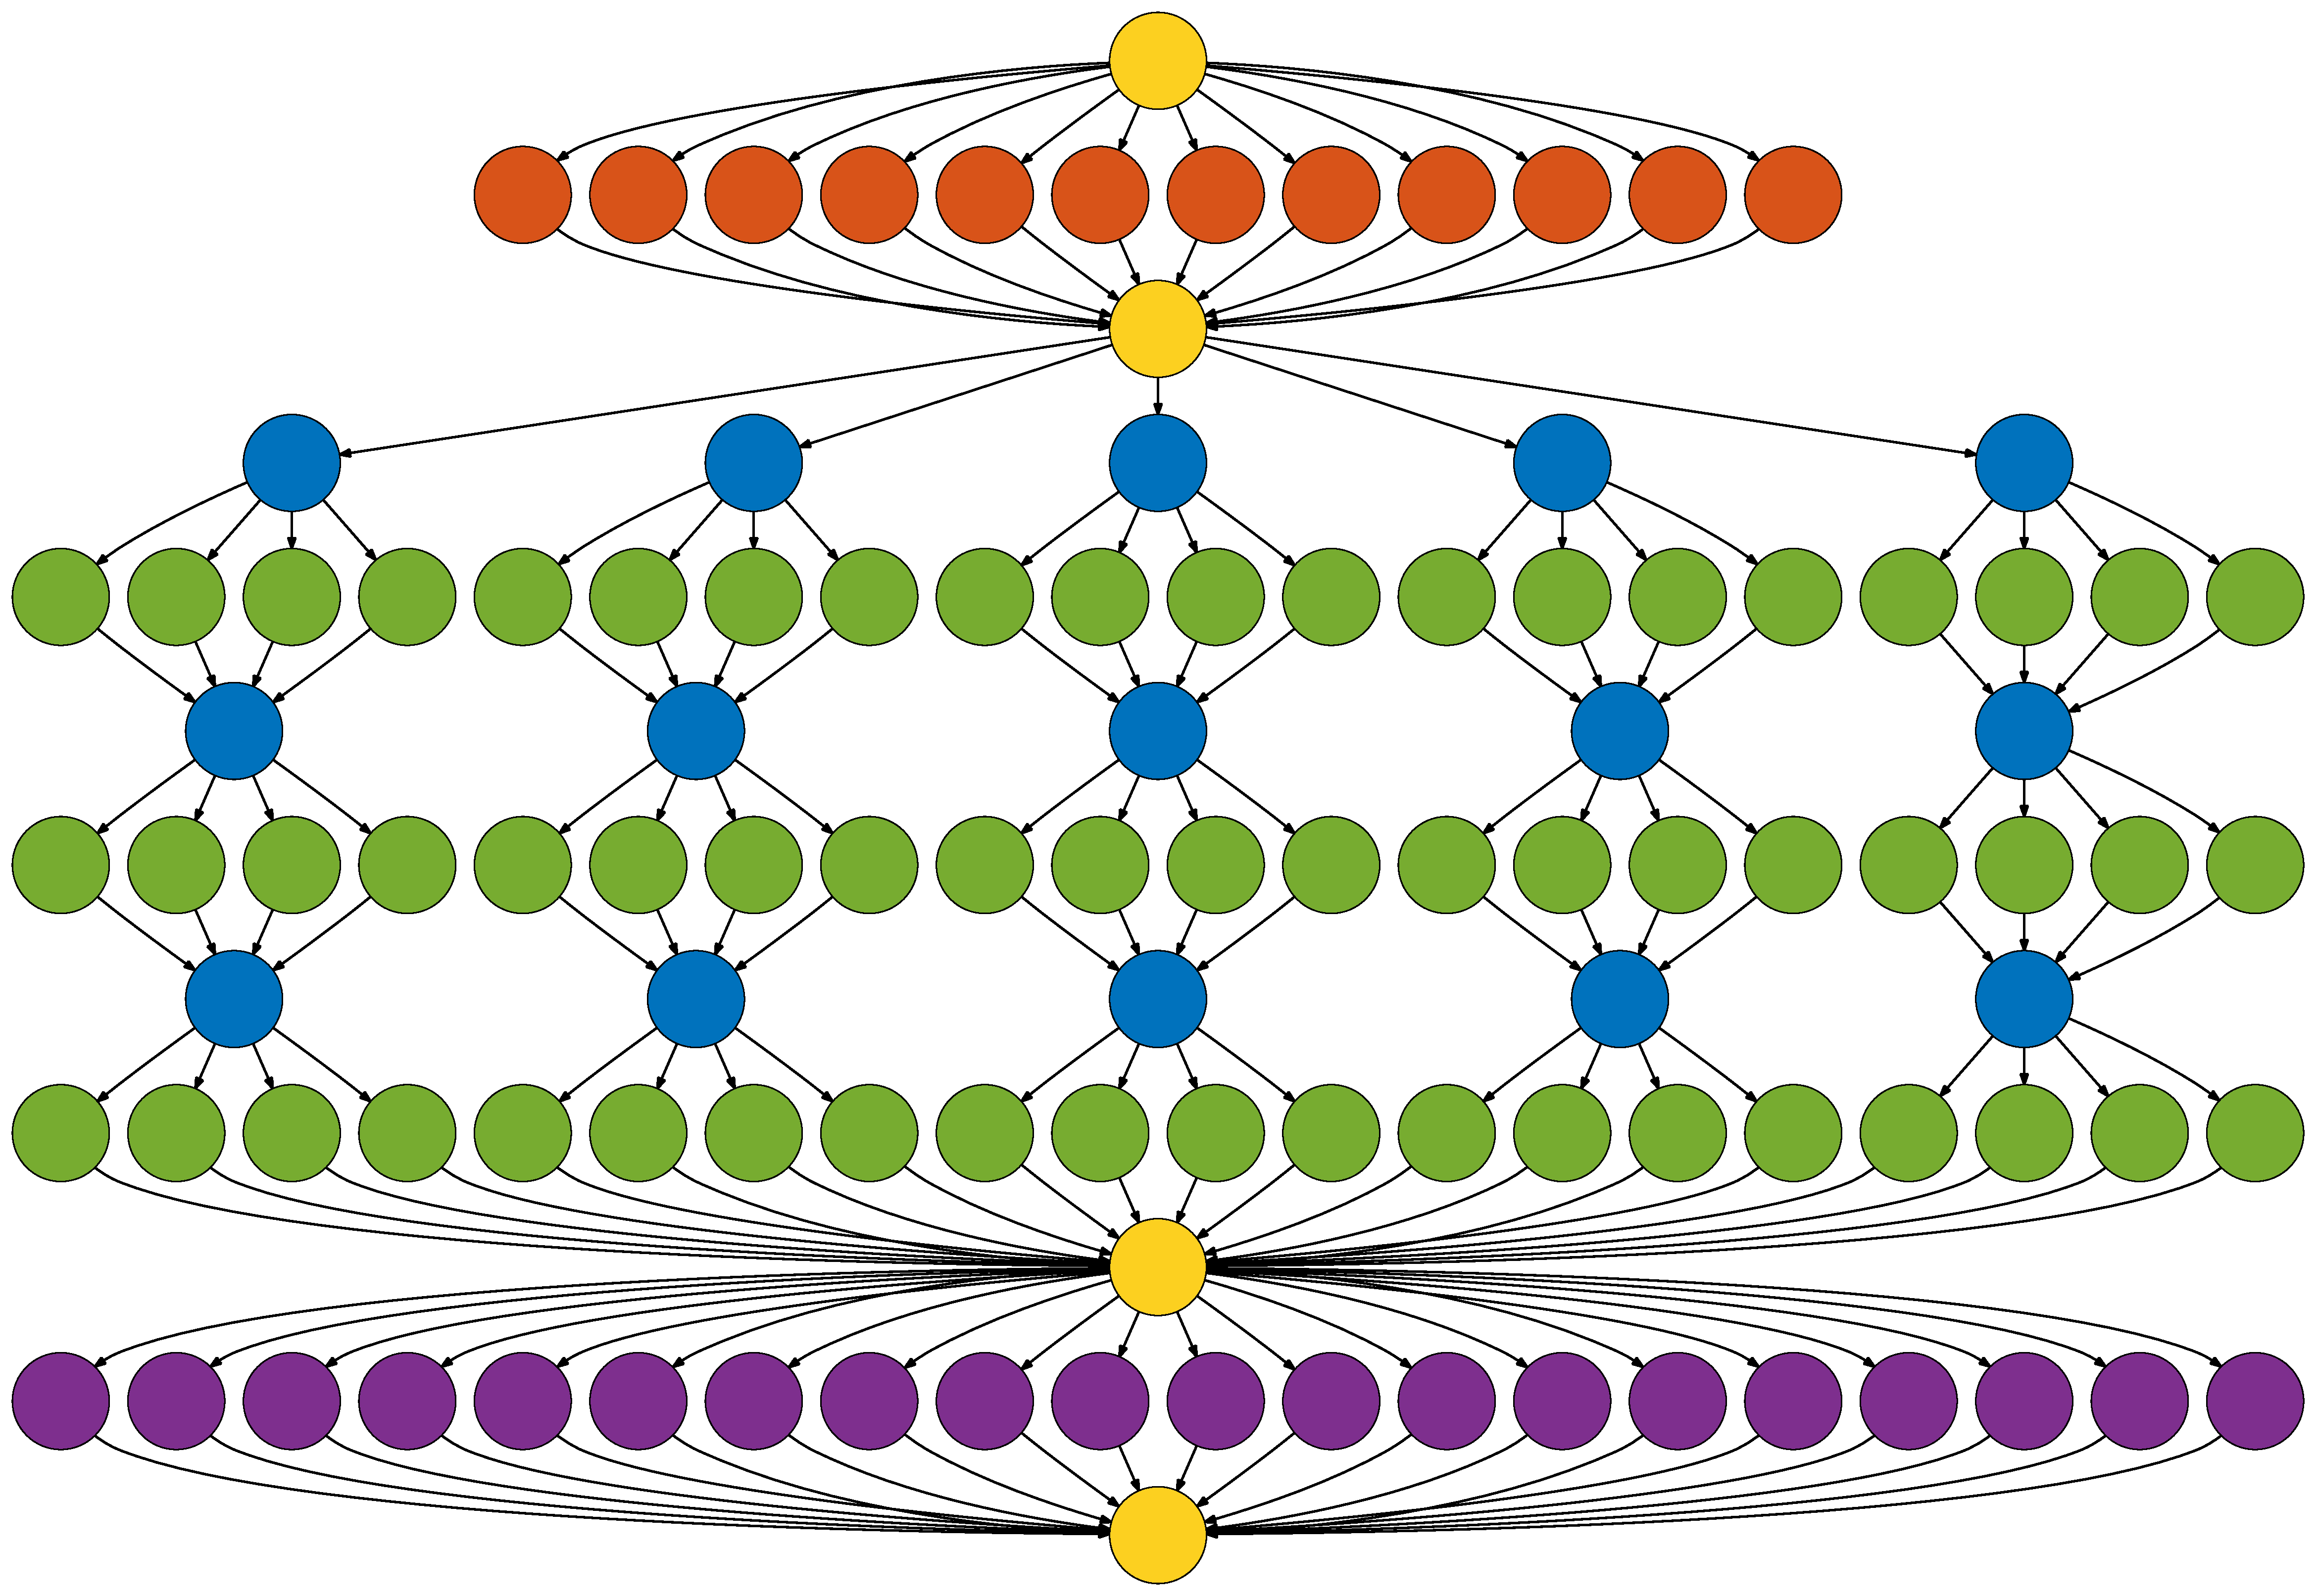
\includegraphics[width=0.95\columnwidth]{fig/deps}
    \end{center}
    \caption{Task dependencies of a convolutional layer.}
    \label{fig:task_deps}
  \end{figure}

  The main quantities of the task parallel algorithm are: (1) breaking
  up the computation required by the convolutional layer into tasks
  that operate on an independent chunk of memory, (2) creating a task
  dependency graph, and (3) scheduling the tasks for execution.

  There are five different task types:

  \begin{itemize}
    \item {\color{zred}\bf Input image transform} task computes the
      forward FFT transform of a single input image.
    \item {\color{zblue}\bf Kernel transform} task computes the forward
      FFT transform of a single kernel.
    \item {\color{zgreen}\bf Multiply-add} task computes the
      point-wise product of an input image and a kernel FFT
      accumulating the result to an appropriate image transform.
    \item {\color{zpurple}\bf Output image transform} task computes
      the inverse FFT of the appropriate accumulated image transform.
      This task is also responsible for adding the bias and applying
      the transfer function.
    \item {\color{zyellow}\bf Synchronization} tasks, beside serving
      as synchronization points are the only tasks responsible (and
      only ones allowed) to allocate and/or deallocate memory.
  \end{itemize}

  {\color{zblack}}

  The task dependency graph of all the tasks required for computing
  the output images of a convolutional layer with four input and five
  output feature-maps for an input mini--batch size of $4$ is shown on
  Figure~\ref{fig:task_deps}.  The tasks are created and queued when
  all their dependencies have been satisfied.  There are four
  {\color{zyellow}\bf synchronization} tasks effectively dividing the
  computation into three stages.  The layout of the {\color{zblue}\bf
    kernel transform} tasks forms a grid, with the number of columns
  equal to the number of output feature-maps, and the number of rows
  equal to the number of input feature-maps.  The task of the $i$th
  column and $j$th row computes the transform of the kernel $w_{i,j}$.
  Furthermore, each such task has $S$ dependent {\color{zgreen}\bf
    multiply-add} tasks, where $S$ is the batch size of the input
  (equal to four in Figure~\ref{fig:task_deps}).  The $k$th dependent
  {\color{zgreen}\bf multiply-add} task of a {\color{zblue}\bf kernel
    transform} task in column $i$ and row $j$ accumulates the product
  of the transforms of the $j$th input image of the $k$th batch and
  the filter $w_{i,j}$ to the transform of the $i$th output image of
  the $k$th batch.

  The tasks are executed by $N$ worker threads, where $N$ equals the
  number of available cores (or virtual cores, when hyper--threading
  is enabled).  Each worker thread is {\bf pinned} to a single core,
  meaning that it can be executed on a specific hardware core.  For
  this reason, we will use ``worker thread'' and ``core''
  interchangeably.

  The first {\color{zyellow}\bf synchronization} task allocates memory
  for the FFT transforms of the input images.  The number of dependent
  {\color{zred}\bf input image transform} tasks equals the number of
  input feature-maps times the mini--batch size $S$.  They are then
  executed by the $N$ worker threads, such that each worker picks up
  an arbitrary task and executes it.

  The last thread to complete the execution of an {\color{zred}\bf
    input image transform} task immediately executes the second
  {\color{zyellow}\bf synchronization} task.  This tasks deallocates
  the memory holding the input images, as their values are no longer
  required. It then allocates memory for the transforms of the output
  images.  At this point $M$ threads are chosen as \emph{primary}
  threads, where $M$ is the maximum of $N$ -- total number of threads,
  and the number of output feature--maps.  The \emph{primary} threads
  are chosen so that they are evenly distributed over multiple
  physical chips.  Each \emph{primary} thread is given a temporary
  buffer equal to the size required to fit the transform of a padded
  kernel for that layer.

  The {\color{zblue}\bf kernel transform} tasks and {\color{zgreen}\bf
    multiply-add} tasks are then scheduled for execution based on
  their distance to the sink node of the task dependency graph, such
  that the more distant nodes get scheduled first.  The scheduling has
  two additional constraints: (1) the {\color{zblue}\bf kernel
    transform} tasks can only be executed by a \emph{primary} thread,
  and (2) its dependent {\color{zgreen}\bf multiply-add} tasks can
  only be executed by worker threads that are pinned to the same
  physical chip.

  This strategy is chosen over the popular alternative approach to
  task scheduling based on work stealing~\cite{reinders2007intel,
    willhalm2008putting} because it divides the work more evenly over
  multi-chip machines and further increase cache locality.  On a 4-way
  machine it yields more deterministic results -- very little variance
  in run-time and average of 20\% speed improvement over the
  alternative.

  The last {\color{zgreen}\bf multiply-add} task to complete executes
  the third {\color{zyellow}\bf synchronization} task.  This task
  deallocates the memory buffers given to the primary threads as well
  as the memory used to store the transforms of the input images.  It
  also allocates the memory to store the final result -- the output
  images.

  The number of {\color{zpurple}\bf output image transform} tasks
  equals the number of output feature-maps times the batch size.  The
  tasks are executed by all $N$ workers, such that each worker picks
  up an arbitrary task and executes it.  The last {\color{zpurple}\bf
    output image transform} task to finish also executes the final
  {\color{zyellow}\bf synchronization} task, which frees the memory
  required for the output image transforms.

  The task parallel algorithm requires that both $f \cdot S$ and $f'
  \cdot S$ be large enough (at least the same size as the number of
  available cores) in order to efficiently utilize all the cores.  In
  such cases they can be much more efficient than the data parallel
  algorithm, as the tasks operate on independent data (thus reducing
  false--sharing, a case where one CPU's cache is invalidated because
  multiple CPUs operate on adjacent memory).  It further improves the
  performances on multi--chip systems, by minimizing the data sharing
  between cores on different chips. On a 4--way Intel Xeon E7--8890 v3
  machine the task parallel algorithm is $10 \times$ faster than the
  data parallel one (for large enough $f' \cdot S$ and $f \cdot S$).

  As shown later, this is the implementation that is optimal in most
  cases, even for very small kernel sizes; the only exception is the
  first layer of the network for which both $f = 1$ and $S = 1$.

  The memory required by the task parallel algorithm can be higher
  then the one of the data parallel algorithm, when many cores are
  available.  The exact memory required equals to the maximal memory
  required by each of the 3 stages, and is given in
  Table~\ref{table:memory_requirements}.


\subsection{GPU implementations}

  For the GPU, we propose three different algorithms.  Two of them use
  based on cuDNN's 3D convolution that are based on implicit
  matrix--matrix multiplication.  The third FFT--based implementation
  is based on our, previously described, algorithm for padded--pruned
  FFTs.

\subsubsection{Direct convolution using cuDNN}

  The two algorithms using the direct convolution are implemented
  using cuDNN.  CuDNN performs 3D convolution as an implicit
  matrix--matrix multiplication, meaning that the matrices are not
  actually created.  The first algorithm improves the speed by
  pre--computing a set of indices, and thus require additional
  workspace memory.  The second algorithm, which we find 3-5$\times$
  slower does not require any extra memory.

\subsubsection{FFT based algorithm}

  FFT-based convolutional layer is based on the GPU implementation of
  the padded--pruned FFT algorithm adescribed in
  Section~\ref{sec:gpu-fft-impl}.

  \begin{algorithm}
    {\small
    \begin{codebox}
      \Procname{$\proc{Convolutional-Forward-FFT-GPU}(I,w,S,f,f',\vec{n},\vec{k})$}
      \li $\vec{n}' = \vec{n} - \vec{k} + \vec{1}$
      \li $\widetilde{I} \gets \proc{5D-Complex-Tensor}(S,f,\floor{n_x/2}+1,n_y,n_z)$
      \li $\widetilde{s} \gets \proc{5D-Complex-Tensor}(f,\floor{n_x/2}+1,n_y,n_z)$
      \li \For $i \gets 0 \To S-1$
      \li   \Do $\widetilde{I}_{i} \gets \proc{GPU-Parallel-FFT}(I_{i},\widetilde{s})$
      \End
      \li $\proc{Free-Memory}(I)$
      \li $\widetilde{O} \gets \proc{5D-Complex-Tensor}(S,f',\floor{n_x/2}+1,n_y,n_z)$
      \li \For $i \gets 0 \To f'-1$
      \li    \Do $\widetilde{w}_{i} = \proc{Parallel-FFT}(w_{i},\widetilde{s})$
      \li        \For $j \gets 0 \To S-1$
      \li           \Do $s \gets \proc{Parallel-Mult}(\widetilde{w}_{i}, \widetilde{I}_{j})$
      \li               $\widetilde{O}_{j,i} \gets \proc{Parallel-Accumulate}(s)$
      \End \End
      \li $\proc{Free-Memory}(\widetilde{I})$
      \li $\proc{Free-Memory}(\widetilde{s})$
      \li $O \gets \proc{5D-Real-Tensor}(S,f',n'_x,n'_y,n'_z)$
      \li $\widetilde{s} \gets \proc{5D-Complex-Tensor}(f',\floor{n_x/2}+1,n_y,n_z)$
      \li \For $i \gets 0 \To S-1$
      \li   \Do $O_{i} \gets \proc{GPU-Parallel-Inverse-FFT}(\widetilde{O}_{i})$
      \End
      \li $\proc{Free-Memory}(\widetilde{O})$
      \li $\proc{Free-Memory}(\widetilde{s})$
      \li \Return $O$
    \end{codebox}
    }

    \caption{FFT based convolutional layer algorithm for the GPU.}
    \label{alg:gpu_alg}
  \end{algorithm}

  The algorithm, given in Algorithm~\ref{alg:gpu_alg} resembles the
  task based CPU algorithm in the sense that it has three main stages
  with memory allocated/deallocated between the stages.  The lines 2
  and 3 allocate memory required for the input image transforms and
  the scratch space required by $\proc{GPU-Parallel-FFT}$ procedure
  explained in Section~\ref{sec:gpu-fft-impl}.  The first stage (lines
  4 and 5) computes the transforms of all the input images by
  performing $f$ 3D FFTs in parallel.  The memory used by the input
  images is then released, and memory for storing the FFTs of the
  output images is allocated (lines 6 and 7).

  In the second stage (lines 8--12) we loop over the $f'$ output
  feature-maps.  For each output feature--map we compute the transform
  of the $f$ relevant kernels (ones connecting each of the input
  feature--maps and the current output feature--map).  We then loop
  over the mini--batches, and for each mini--batch we compute the
  point--wise product of the relevant input image transforms with the
  relevant kernel transforms, producing $f$ complex valued images.
  The values of the $f$ images are then accumulated to a single image,
  -- the transform of the appropriate output image.  Note how we can
  re--use the scratch space $s$ (used for $\proc{GPU-Parallel-FFT}$)
  to store the point--wise product of $f$ transformed images.

  The memory used by the input image transforms, and the scratch space
  is then released.  We then allocate memory for the output images as
  well as new scratch space of different size, required for computing
  $f'$ inverse FFT transforms at once (lines 13--16).

  In the final stage (lines 17 and 18) we compute the output images by
  looping over the mini--batches and computing $f'$ inverse FFTs in
  parallel.  Finally we free the memory of the output transforms and
  the scratch space.

  The memory required by the algorithm is equal to the maximum of
  memory required in each of the three stages
  (Table~\ref{table:memory_requirements}).

\subsection{GPU + host RAM implementation}

  \begin{figure}
    \centering
    \subfloat[]{\protect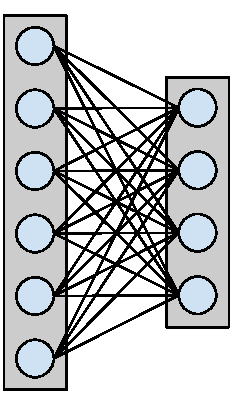
\includegraphics[width=0.08\textwidth]
      {fig/gpuram1.pdf}
      \label{fig:partial_execa}
    }
    \subfloat[]{\protect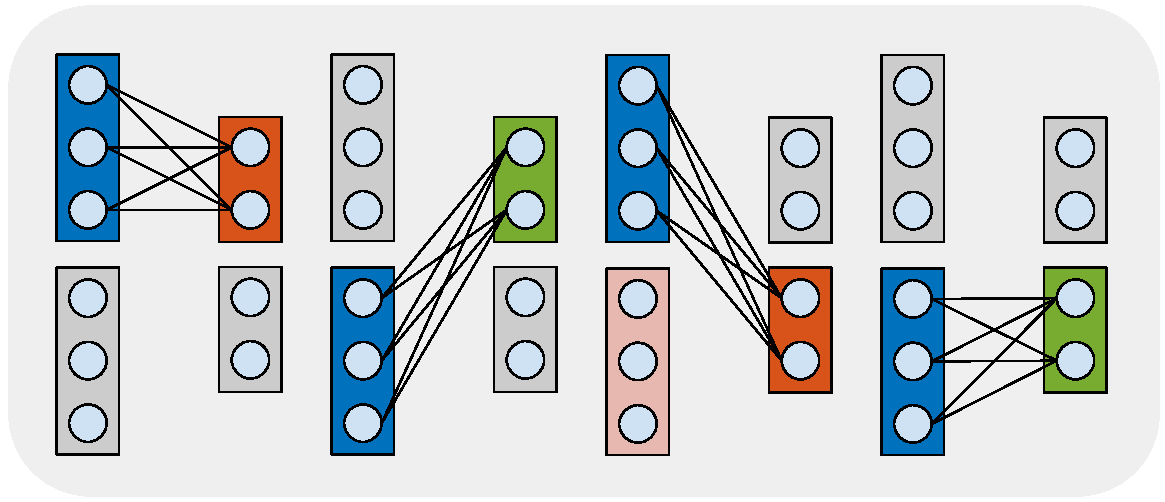
\includegraphics[width=0.36\textwidth]
      {fig/gpuram2.pdf}
      \label{fig:partial_execb}
    }
    \caption{Decomposing a convolutional layer into multiple
      convolutional sub--layers.}
    \label{fig:partial_exec}
  \end{figure}

  The memory requirements of the GPU algorithms described above limit
  the size of the layer's input.  It turns out that it is useful to be
  able to process large inputs that might fit the host RAM but not the
  GPU's on--board RAM.

  In such cases we can have the following two scenarios: (1) The
  mini--batch size $S > 1$, and we can process at most $S' < S$ inputs
  on the GPU, and (2) We can't process even a single input on the GPU.

  In the first, case we upload and process a mini--batch of size $S'$
  at the time on the GPU, transferring the result back to the host.
  In the second case, we can still use the GPU by processing one input
  at the time and decomposing the convolutional layer into sub--layers
  (Fig~\ref{fig:partial_exec}). The convolutional layer in
  Figure~\ref{fig:partial_execa} can be decomposed into 4 sub--layers
  that can fit on the GPU RAM (Fig~\ref{fig:partial_execb}). The
  sub--layers can be sequentially executed on the GPU using one of the
  algorithms described above.  The blue color represents the input
  images that has to be transferred to the GPU before the sub--layer
  execution.  The red color represents the memory that has to be
  allocated on the GPU before the execution.  Finally, the green color
  represent that fully computed output images that will be transferred
  to the host after the sub--layer execution.

  The optimal way to decompose a layer into sub layers depends on
  three main factors -- memory transfer speed, the size of the
  input/output 3D images, the GPU's on--board RAM available, and the
  choice of algorithm for each sub--layer.  Generally, for small
  kernel sizes, the direct convolution algorithm should be used, and
  for larger kernels, the FFT--based algorithm.  Determining the
  optimal sub--layer sizes is a much more complex problem, but can
  easily be chosen empirically.

  The host memory requirement for this layer equals to the amount of
  memory required to store the input and the output tensor.  The GPU
  on--board memory has to be large enough to perform the finest
  granularity sub--layer, which is essentially a single image
  convolution -- enough memory to store one input 3D image, a kernel,
  and one output 3D image.

\section{Algorithms for the max--pooling and MFP layers}

  \emph{Max pooling} of an image of size $\vec{n}$ with the window
  size of $\vec{p} = (p_x,p_y,p_z)$ divides an image into blocks of
  size $\vec{p}$.  The maximum value is computed for each block,
  yielding an image of size $(n_x/p_x,n_y/p_y,n_z/p_z)$.  The input
  image size $\vec{n}$ is restriceted such that $n_x$, $n_y$ and $n_z$
  are divisible by $p_x$, $p_y$ and $p_z$ respectively.

  On the CPU, we implement the max--pooling layer so that the
  max--pooling of each image is performed in parallel (e.g. by using
  parallel for loop).  For the GPU we use the cuDNN primitives for
  max--pooling.

  \emph{Max fragment pooling} of an image of size $\vec{n}$ with the
  window size of $\vec{p}$ produces $p_x \times p_y \times p_z$ output
  images (fragments) by performing multiple \emph{max pooling}
  operations on the image at offsets $(x,y,z)$, where $0 \le x < p_x$,
  $0 \le y < p_y$, and $0 \le z < p_z$.  When the image has size such
  that $\vec{n} + \vec{1}$ is divisible by $\vec{p}$, the sizes of all
  produced fragments will equal
  $(\floor{n_x/p_x},\floor{n_y}{p_y},\floor{n_z}{p_z})$.

  Similarly as in the max--pooling case, our CPU implementation loops
  over all the $f$ input images of each of $S$ inputs in a parallel
  for loop, and performs the MFP by performing the
  max--pooling operation at each offset.

  The GPU implementation is based on the cuDNN primitive for
  max--pooling.  For each valid offset $(x,y,z)$ we invoke the cuDNN
  max--pooling primitive to compute the max--pooling of all the input
  images at that offset.



\section{ConvNet computation strategies}

  \begin{figure}
    \centering
    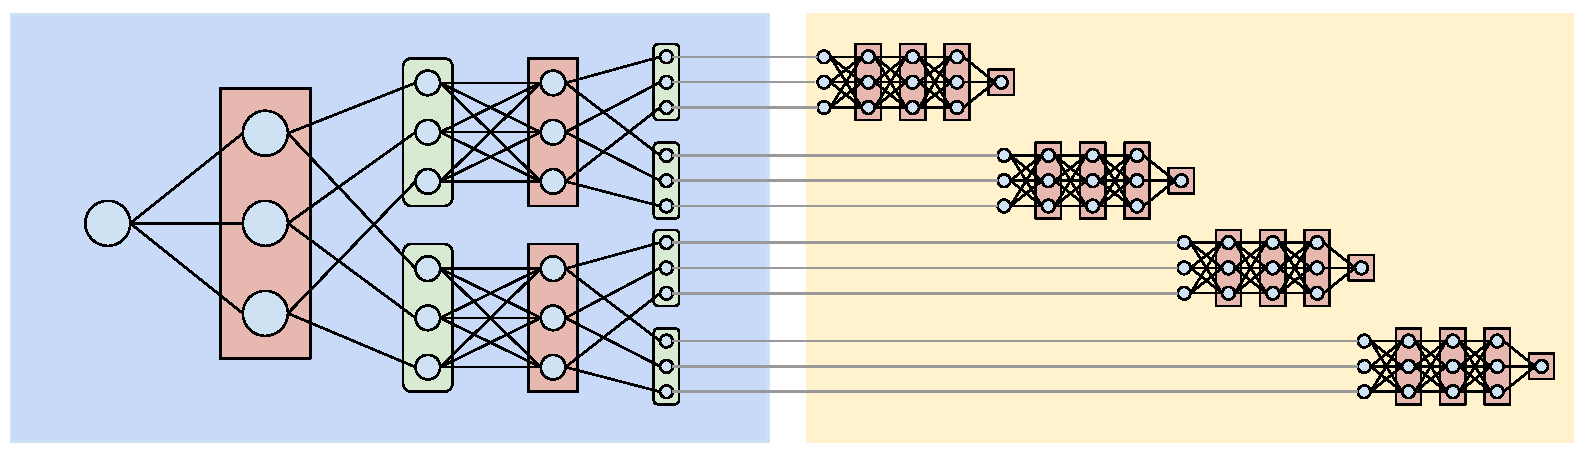
\includegraphics[width=0.99\columnwidth]{fig/layer_vs_batch.pdf}
    \caption{Layer at the time vs mini--batch at the time execution.}
    \label{fig:executions}
  \end{figure}

  For a given ConvNet and a mini--batch of $S$ inputs, the ConvNet
  output can be computed in two different ways -- a layer at the time,
  or a mini--batch at the time.

  In the first case we sequentially perform the computation for each
  layer of the network on all given inputs.  The input shape of each
  layer will equal to the output shape of the previous layer, as given
  in Table~\ref{table:layers_complexity}.  This strategy allows for
  re--use of the kernel FFTs, and better potential for parallelization
  on the GPU, as more outputs are computed at the same time.  The
  memory required by this approach is equal to the maximal memory
  required of each layer.

  The second strategy is to apply the network on a $S' < S$ inputs at
  the time.  This approach

\subsection{Sparse vs dense output}

  As described in~\ref{sec:sliding-window} the two ways to produce an
  output of a sliding--window ConvNet is by: (1) naively applying a
  max--poling ConvNet for every window location and (2) using
  \emph{MFP} or \emph{filter-rarefication}.
  The second approach greatly reduces the amount of computation
  required per output pixel~\cite{giusti2013fast,masci2013fast,
    zlateski2015znn,long2015fully,sermanet2013overfeat,yu2015multi}.

  It turns out that max--poling networks can be also applied to
  specific input image sizes in order to produce multiple
  \emph{sparse} outputs.  For convenience, the discussion below will
  consider 1D ConvNets, same arguments can be applied to 3D ConvNets.

  A max--pooling ConvNet with a field of view of $v$ and $n$ pooling
  layers each having a window size of $p_i$ can be applied to an input
  images of sizes $(v - 1 + \alpha \prod_{i} p_i)$ producing $\alpha$
  output pixels.  These output pixels represent a sparse output in the
  sense that each pixel had the value of the ConvNet applied to the
  input shifted by $\prod_{i} p_i$.  Therefore, a sliding window
  output of size $\alpha \prod_{i} p_i$ can be computed by performing
  the max--pooling ConvNet computation on $\prod_{i} p_i$ input
  images, each shifted by one pixel.

  \begin{figure}
    \centering
    \subfloat[]{\protect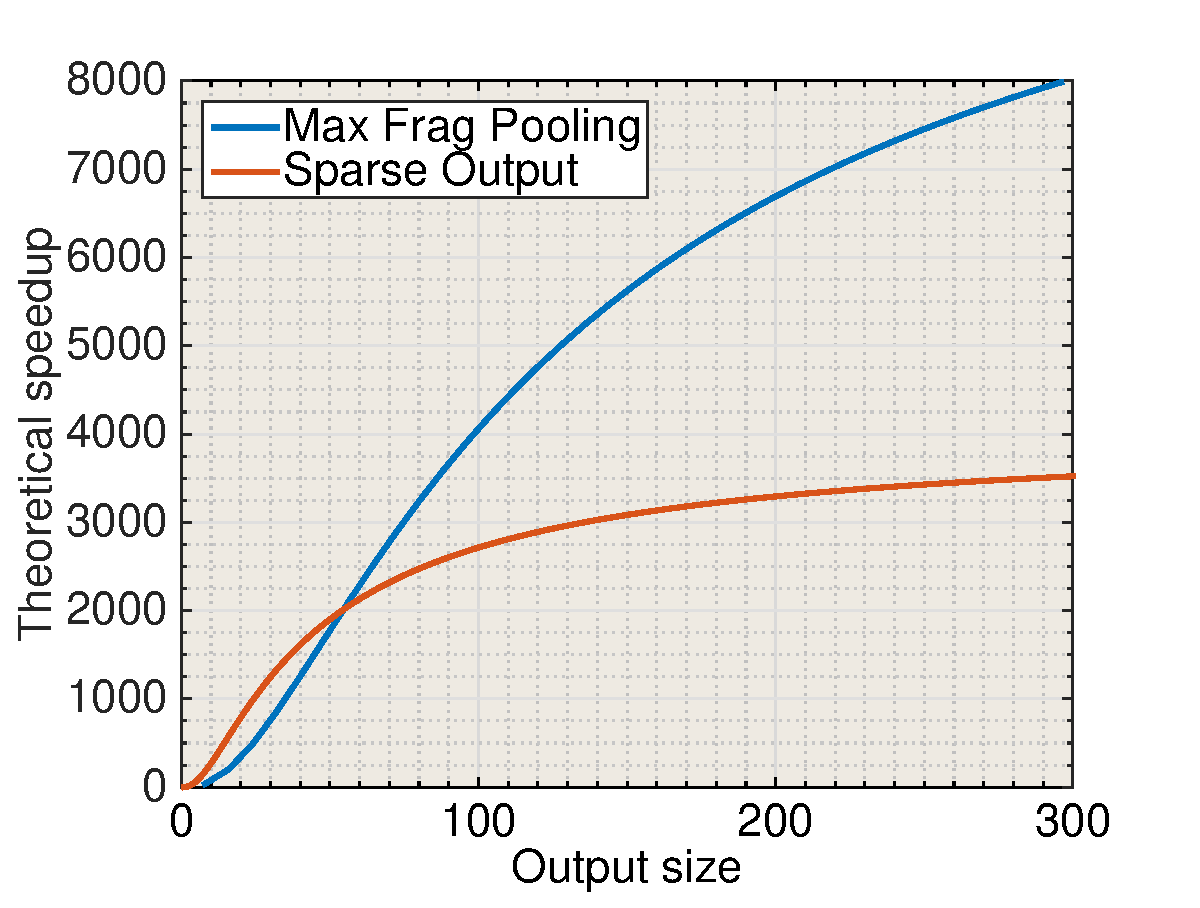
\includegraphics[width=0.24\textwidth]
      {fig/vssparsesize.eps}
      \label{fig:sparse_explanationa}
    }
    \subfloat[]{\protect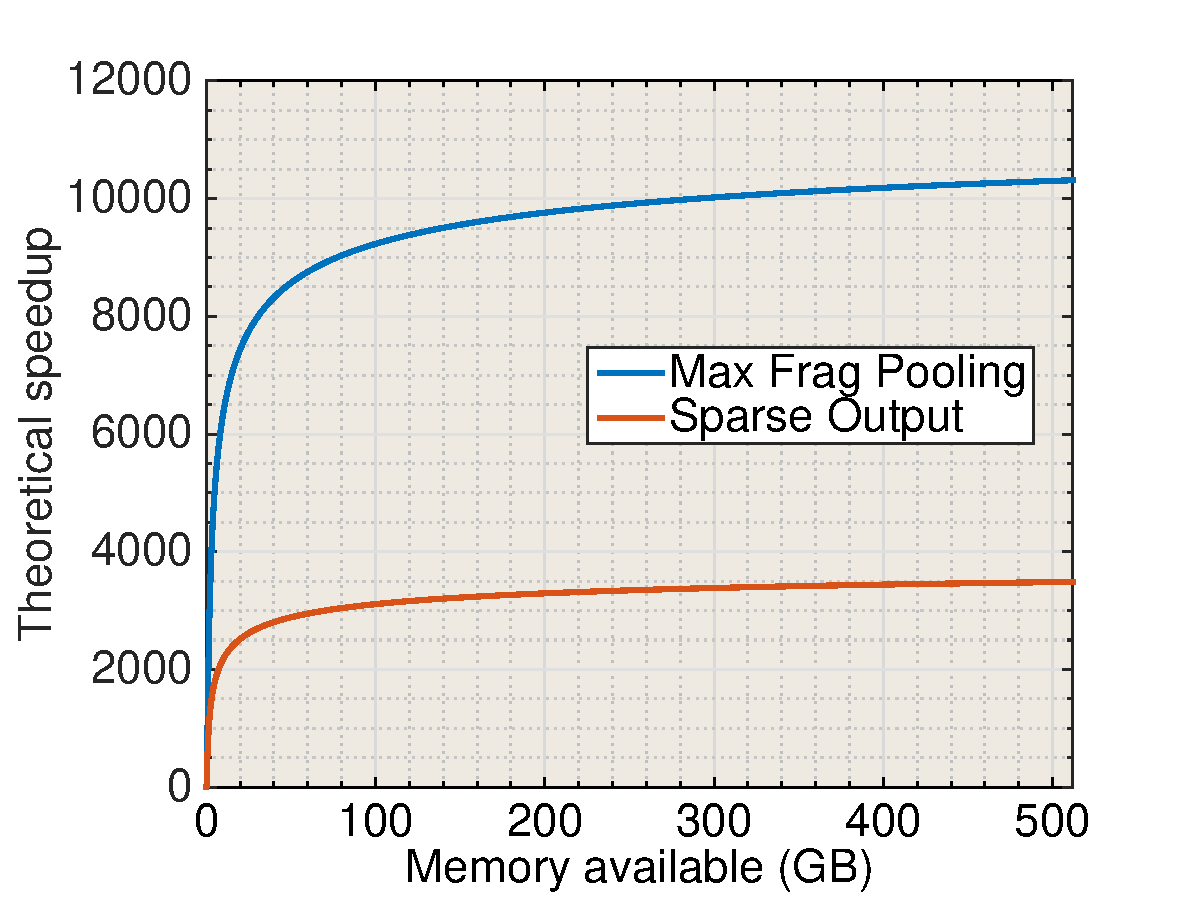
\includegraphics[width=0.24\textwidth]
      {fig/vssparsemem.eps}
      \label{fig:sparse_explanationb}
    }
    \caption{Sparse vs dense.}
    \label{fig:sparse_explanation}
  \end{figure}

  Interestingly, for some fixed output sizes, this approach can
  outperform the \emph{MFP}.
  Figure~\ref{fig:sparse_explanationa} shows the theoretical speedup
  for different output sizes for both \emph{MFP}
  and \emph{sparse} computation as described above.  The theoretical
  speedup is defined as the ratio of operations required for producing
  $1^3$ output vs the amount of operations required per output pixel
  for the given output image size.

  The ConvNet used for Figure~\ref{fig:sparse_explanation} has 2
  pooling layers with the window size of $2^3$ and 6 convolutional
  layers with kernel sizes of $5^3$.  It was assumed that direct
  convolution is used for computation.  Networks with more pooling
  layers and/or different kernel sizes, as well as networks with
  FFT--based convolution show very similar curves -- the \emph{sparse}
  computation achieves better theoretical speedups for some,
  relatively small output sizes.

  When trying to maximize the throughput we are not limited to fixed
  output image size.  As Figure~\ref{fig:sparse_explanationa} suggest
  we should always try to maximize the output image size.  Using
  \emph{sparse} computation for the same output size requires much
  more memory, as the input sizes grow faster than in the
  \emph{MFP} networks.  On
  Figure~\ref{fig:sparse_explanationb} we plot the theoretical speedup
  achievable given certain amount of memory available.  For given
  memory limit we determine what is the largest possible output image
  we can compute using both methods, and plot the theoretical speedup.
  From the figure we can conclude that \emph{MFP}
  always outperforms the \emph{sparse} computation.

\subsection{Optimal mini--batch size for FFT--based convolutions}

  When FFT--based convolution is used increasing increasing the
  mini--batch size $S$ can reduce the required number of operations
  per output pixel, as the FFTs of the kernels can be reused.
  Alternatively FFTs of the kernels can be pre--computed and stored in
  memory~\cite{zlateski2015znn} further reducing the computational
  cost.  Both approaches reduce the amount of operations required for
  computing a single output pixel, while increasing the memory
  requirements for the algorithm.

  \begin{figure}
    \centering
    \subfloat[]{\protect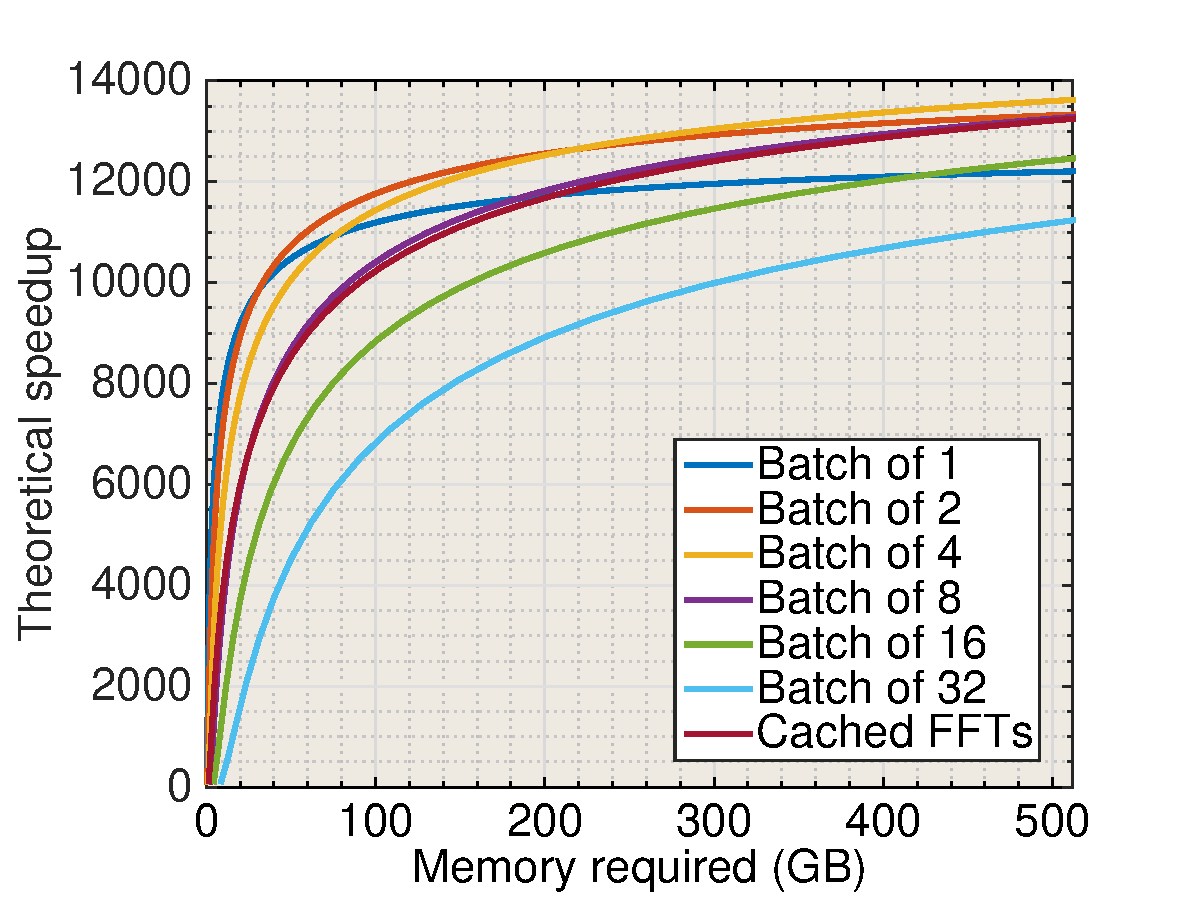
\includegraphics[width=0.24\textwidth]
      {fig/batch1.eps}
      \label{fig:fftbatcha}
    }
    \subfloat[]{\protect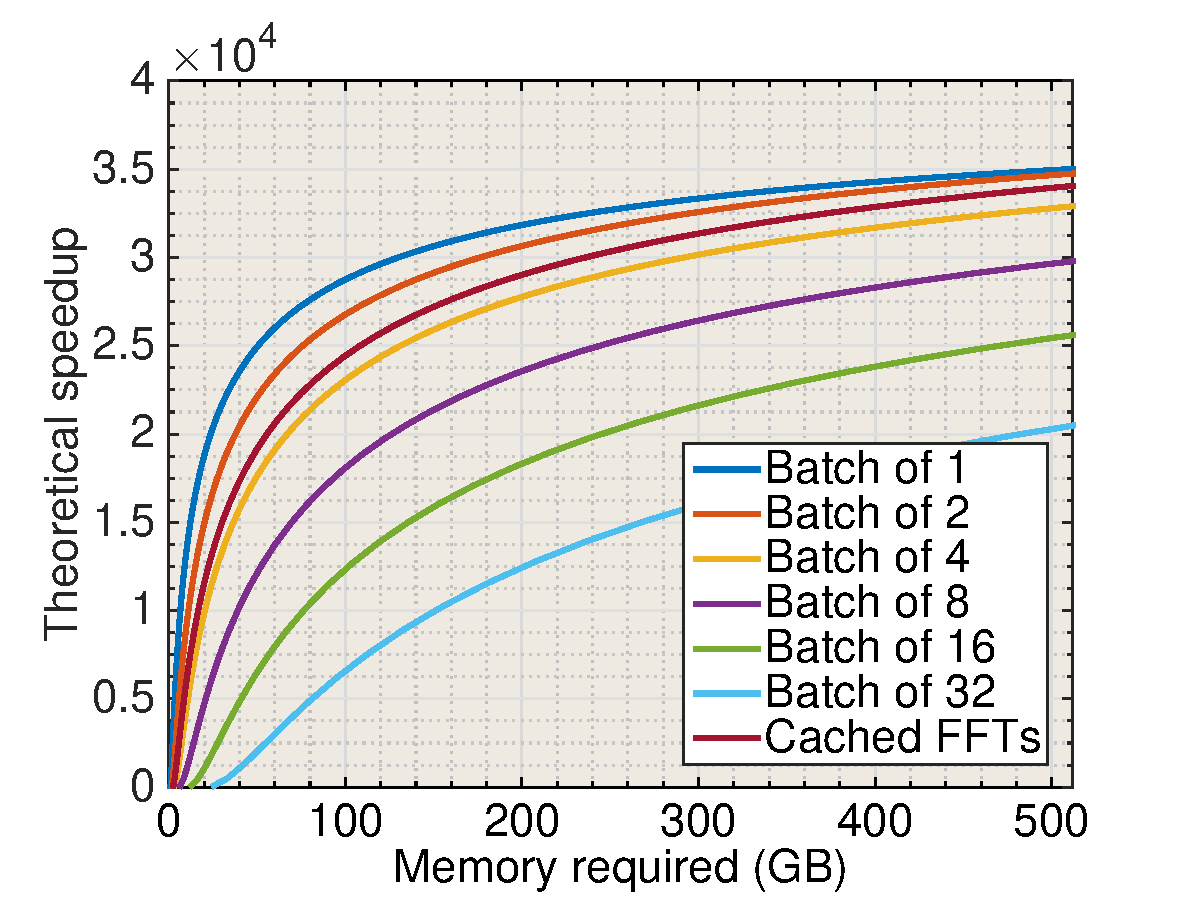
\includegraphics[width=0.24\textwidth]
      {fig/batch2.eps}
      \label{fig:fftbatchb}
    }
    \caption{Batch FFT?.}
    \label{fig:fftbatch}
  \end{figure}

  Explain figure.


\section{Experiments}

  We expect that the performances of our algorithms will strongly
  depend on the ConvNet architecture.  We chose to benchmark the
  throughput of our algorithms on networks with modern architectures
  -- that is, networks with 2 or 3 pooling layers and relatively large
  field of view. (Cite why we think this is a good idea).

  \begin{table}
    \centering
    \begin{tabular}{cccccc}
      \toprule
      Layer & F--maps & n337    & n537  &  n726  &  n926 \\
      \midrule
      $1$ & 80 &  Conv $2^3$  & Conv $4^3$  & Conv $6^3$  & Conv $8^3$ \\
      $2$ & 80 &  Pool $2^3$  & Pool $2^3$  & Pool $2^3$  & Pool $2^3$ \\
      $3$ & 80 &  Conv $3^3$  & Conv $5^3$  & Conv $7^3$  & Conv $9^3$ \\
      $4$ & 80 &  Pool $2^3$  & Pool $2^3$  & Pool $2^3$  & Pool $2^3$ \\
      $5$ & 80 &  Conv $3^3$  & Conv $5^3$  & Conv $7^3$  & Conv $9^3$ \\
      $6$ & 80 &  Pool $2^3$  & Pool $2^3$  & Conv $7^3$  & Pool $9^3$ \\
      $7$ & 80 &  Conv $3^3$  & Conv $5^3$  & Conv $7^3$  & Conv $9^3$ \\
      $8$ & 80 &  Conv $3^3$  & Conv $5^3$  & Conv $7^3$  & Conv $9^3$ \\
      $9$ & 80 & Conv $3^3$  & Conv $5^3$  & & \\
      $10$ & 3 & Conv $3^3$  & Conv $5^3$  & & \\
      \bottomrule
    \end{tabular}
    \caption{ConvNet architectures of the benchmarked networks.}
    \label{table:benchmarked_networks}
  \end{table}


  The large field of view can be accomplished either by having more
  pooling layers or larger filters, for that reason we choose to
  benchmark two networks with seven convolutional layers, and three
  pooling layers ('CPCPCPCCCC') one having filter sizes of $3\times 3
  \times 3$ and the other $5\times 5\times 5$.  Additionally, we
  benchmark two additional networks with 6 convolutional layers and 2
  pooling layers ('CPCPCCCC') with somehow larger filter sizes of $7
  \times 7 \times 7$ and $9 \times 9 \times 9$.  The architectures of
  the benchmarked networks are shown in
  Table~\ref{table:benchmarked_networks}.

  The benchmarks are performed on two machines.  The first machine is
  a 4--way Intel Xeon E7--8890 v3 with total of $72$ cores ($144$
  hyper--threads), 256GB of RAM and a Titan X GPU (with 12GB on--board
  RAM).  The second machine is an Amazon EC2 instance with $32$
  virtual cores and 244GB of RAM (r3.8xlarge).  We use the first
  machine for both GPU--only, CPU--only and CPU--GPU combined
  approaches.  We benchmark the CPU--only approach on the second
  machine as it is much more readily available to general public.


\subsection{GPU--only and CPU--only benchmarks}

  \begin{figure*}[h!t]
    \centering
    \subfloat[]{\protect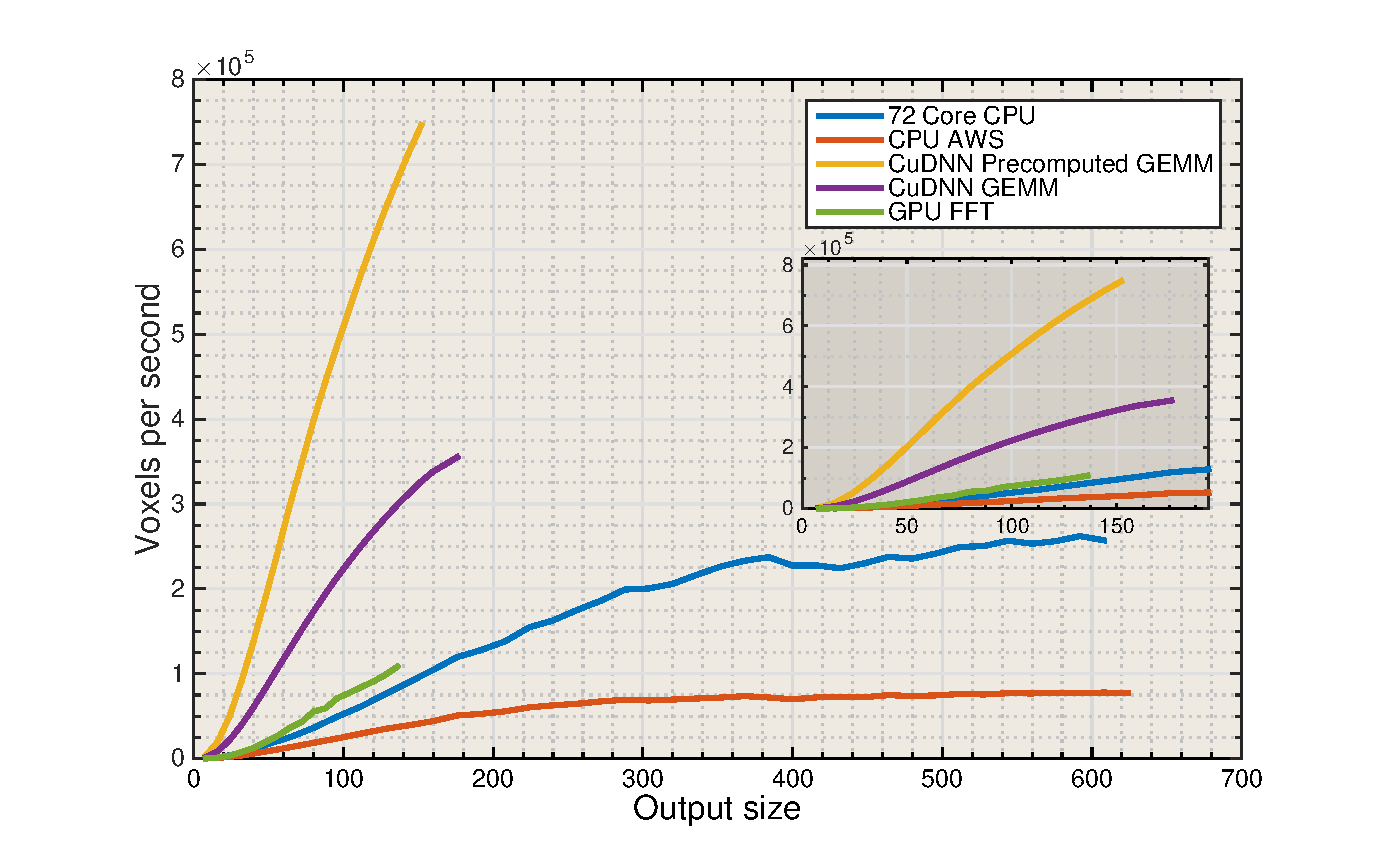
\includegraphics[trim= 15mm 2mm 15mm 5mm, clip, width=0.38\textwidth]
      {fig/m36.eps}}
    \subfloat[]{\protect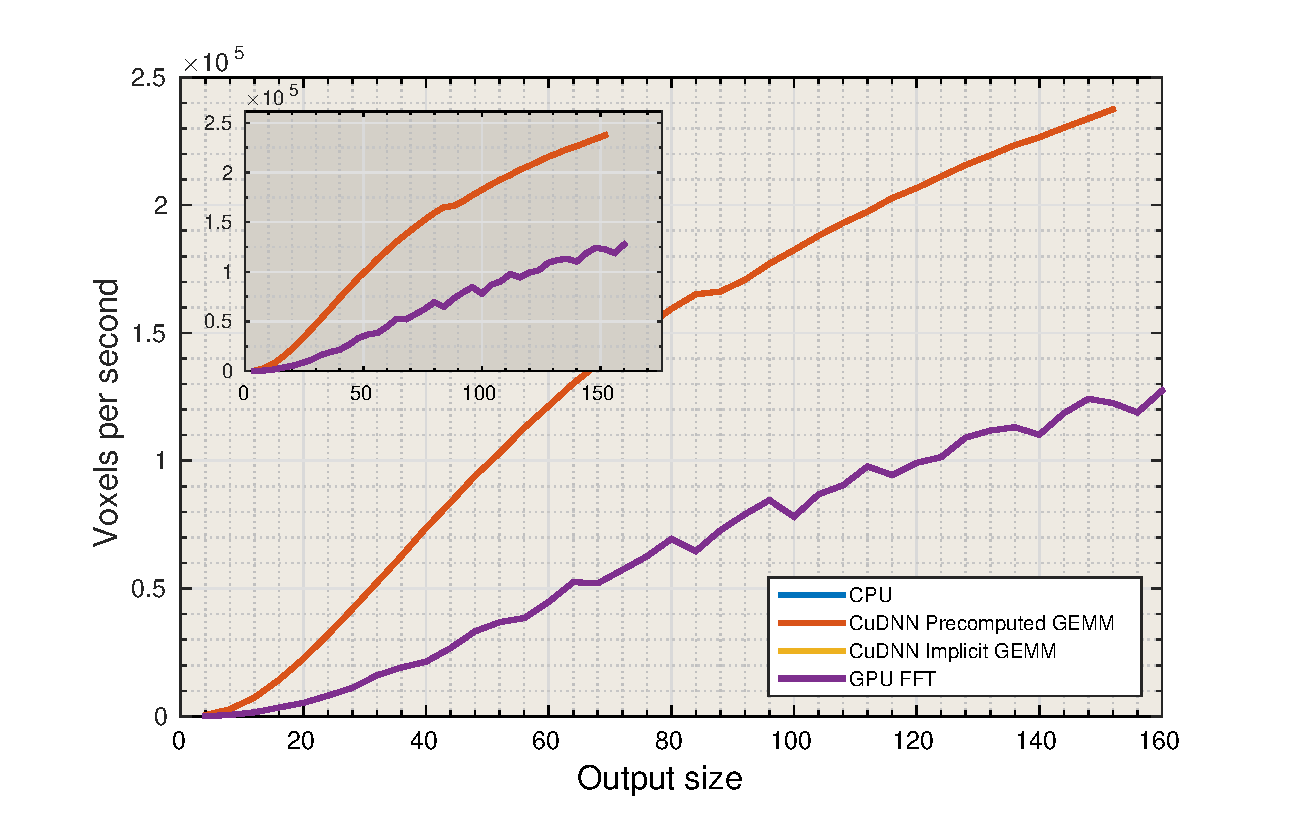
\includegraphics[trim= 15mm 2mm 15mm 5mm, clip, width=0.38\textwidth]
      {fig/m56.eps}}
    \\
    \subfloat[]{\protect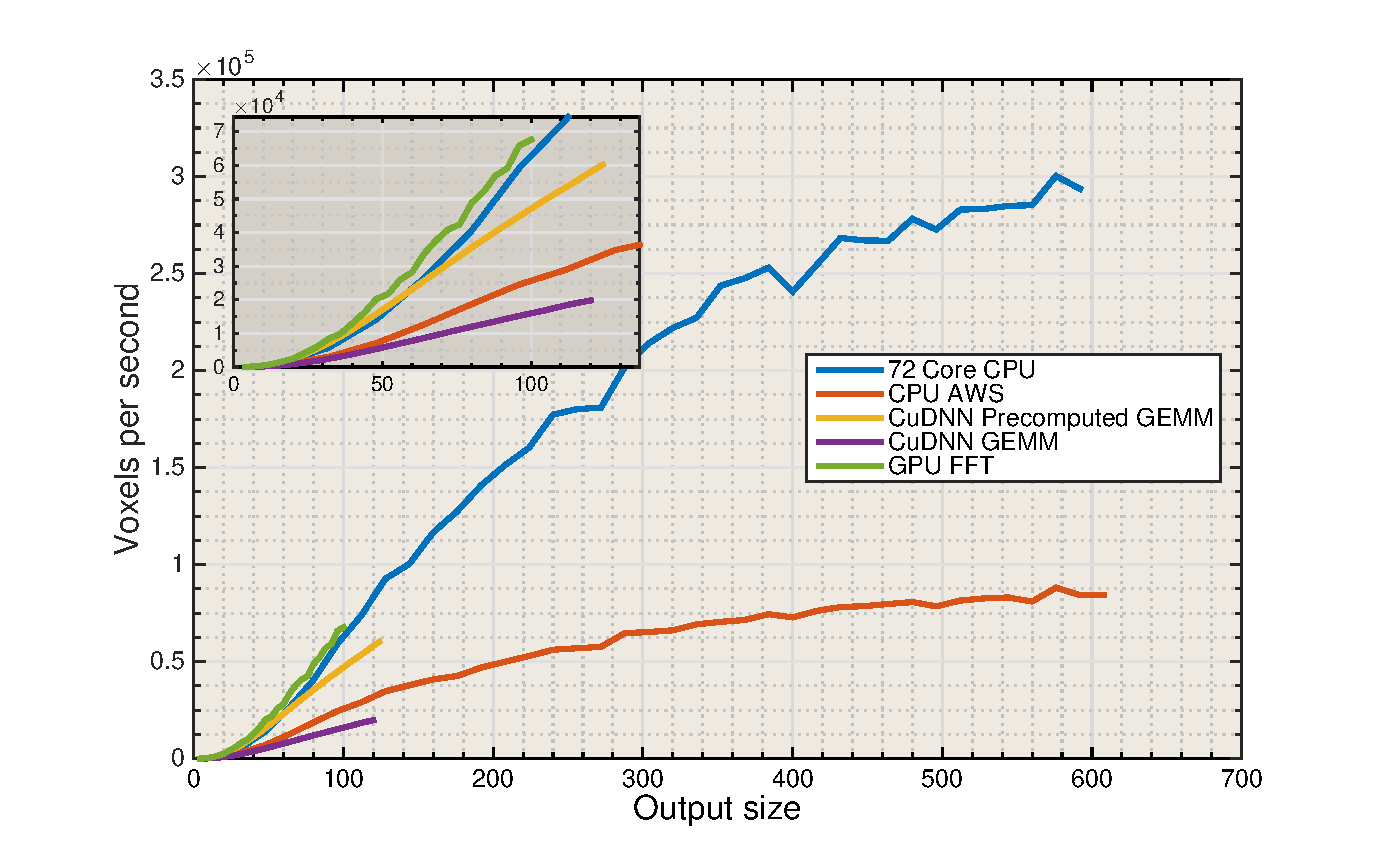
\includegraphics[trim= 15mm 2mm 15mm 5mm, clip, width=0.38\textwidth]
      {fig/m76.eps}}
    \subfloat[]{\protect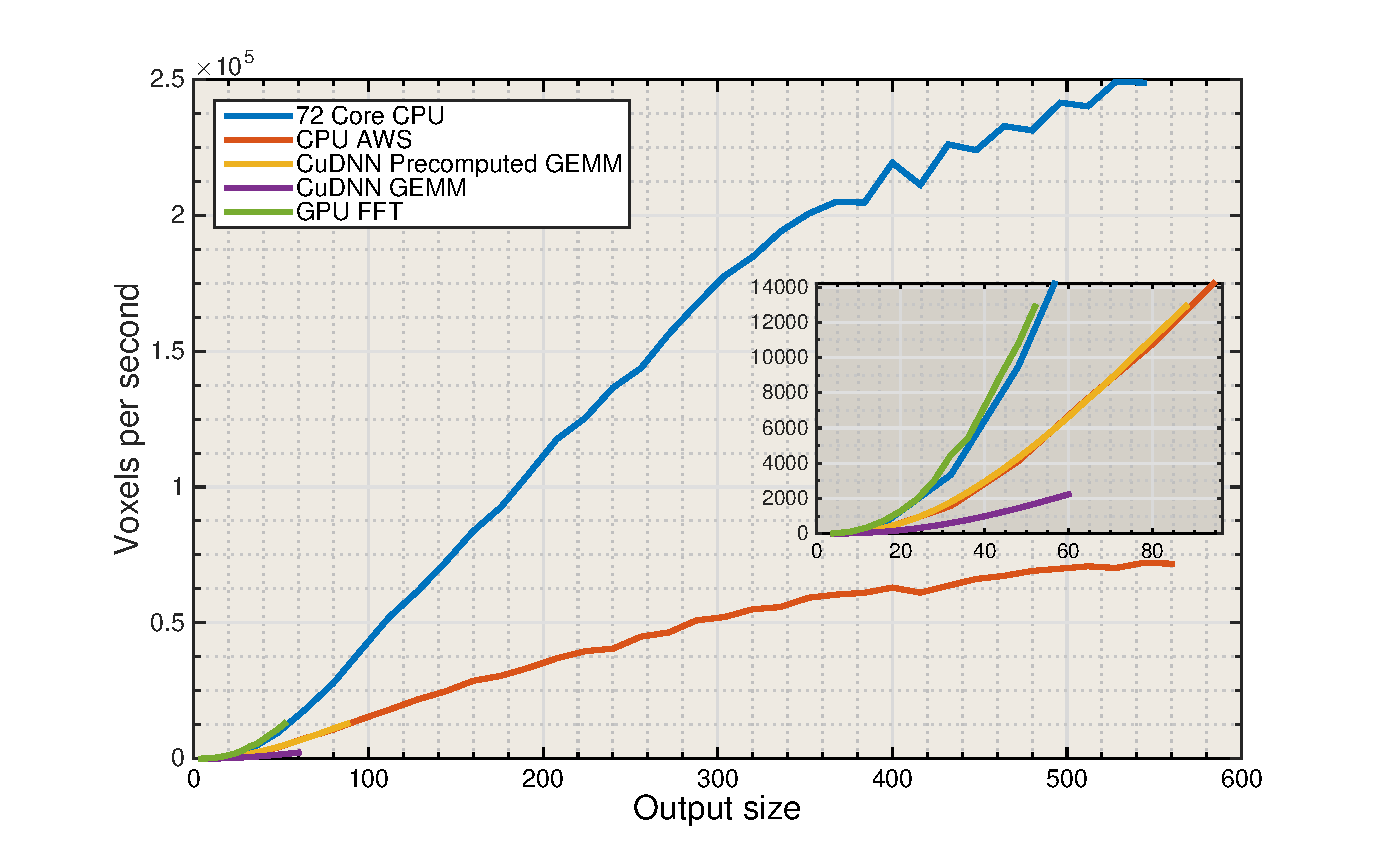
\includegraphics[trim= 15mm 2mm 15mm 5mm, clip, width=0.38\textwidth]
      {fig/m96.eps}}

    \caption{Throughput vs output patch size for pooling networks
    }
    \label{fig:experiments1}
  \end{figure*}

  In our first experiment we benchmark the throughput of the four
  networks using CPU--only and GPU--only network execution.  The
  throughput of each network is shown in
  Figure~\ref{fig:experiments1}.  The three GPU--only implementations
  use the three different convolutional layer algorithms described
  above.  We see that for smaller filter sizes, the direct convolution
  performs better than FFT--based one, and vice versa.

  We measure the CPU--only approaches on two systems (list).  It turns
  out that for CPU--only approaches it is always the best to use the
  task parallel FFT--based algorithm for the convolutional layers,
  except for the first layer, which should be the data parallel
  FFT--based one.  Any other combination of layers always greatly
  under--performs.  For this reason we show only one line per
  benchmarked system.

  We see that for the filter sizes of $7 \times 7 \times 7$ and $9
  \times 9 \times 9$, the GPU--only approach using FFT--based
  convolution and the CPU--only approach on the 72 core machine have
  very similar performances for given output size.  However, due to
  the fact that the CPU has much more available working memory, it is
  able to greatly outperform the GPU--only approach.

  For the filter sizes of $5 \times 5 \times 5$ the GPU--only direct
  convolution outperforms the CPU for a given size, but again, the
  CPUs can achieve higher throughput due to more available RAM.

  The only case where the GPU--only approach outperforms the CPU--only
  approach is for the $3 \times 3 \times 3$ filter sizes.  This is
  expected as for such small filters, direct convolution is much more
  efficient than the FFT--based one, and the GPUs can perform direct
  convolution much more efficiently (cuDNN GEMM).


\subsection{Advanced network execution benchmarks}


  \begin{figure*}[h!t]
    \centering
    \subfloat[]{\protect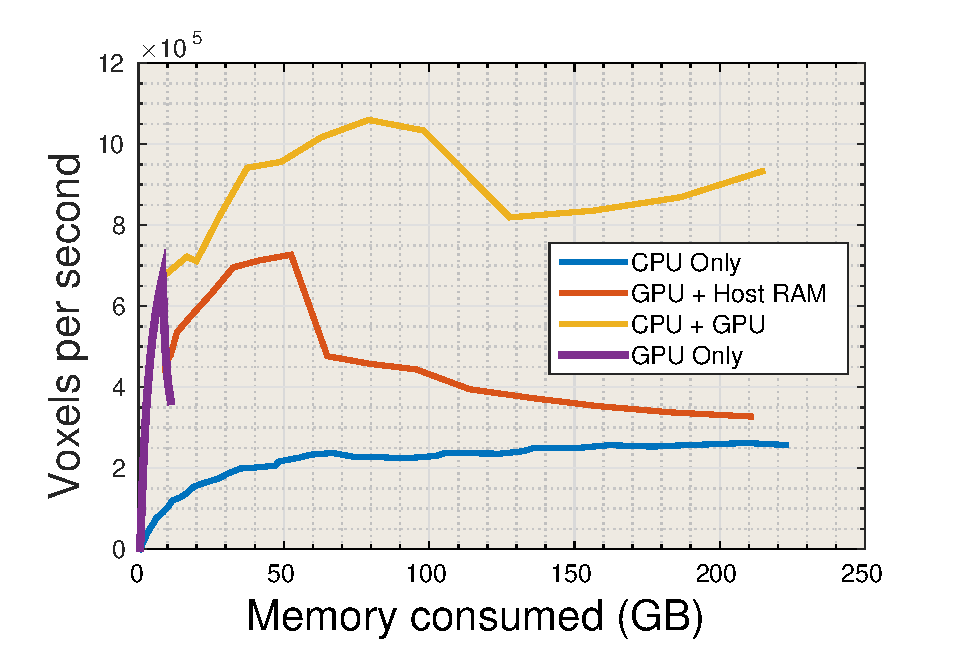
\includegraphics[trim= 10mm 2mm 15mm 5mm, clip, width=0.38\textwidth]
      {fig/m36x.eps}}
    \subfloat[]{\protect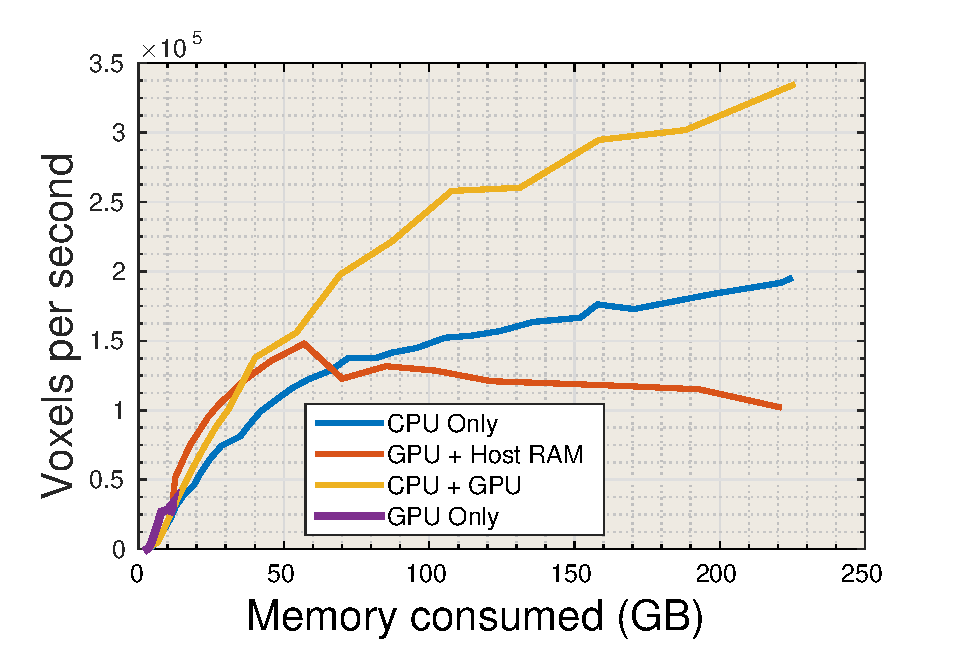
\includegraphics[trim= 10mm 2mm 15mm 5mm, clip, width=0.38\textwidth]
      {fig/m56x.eps}}
    \\
    \subfloat[]{\protect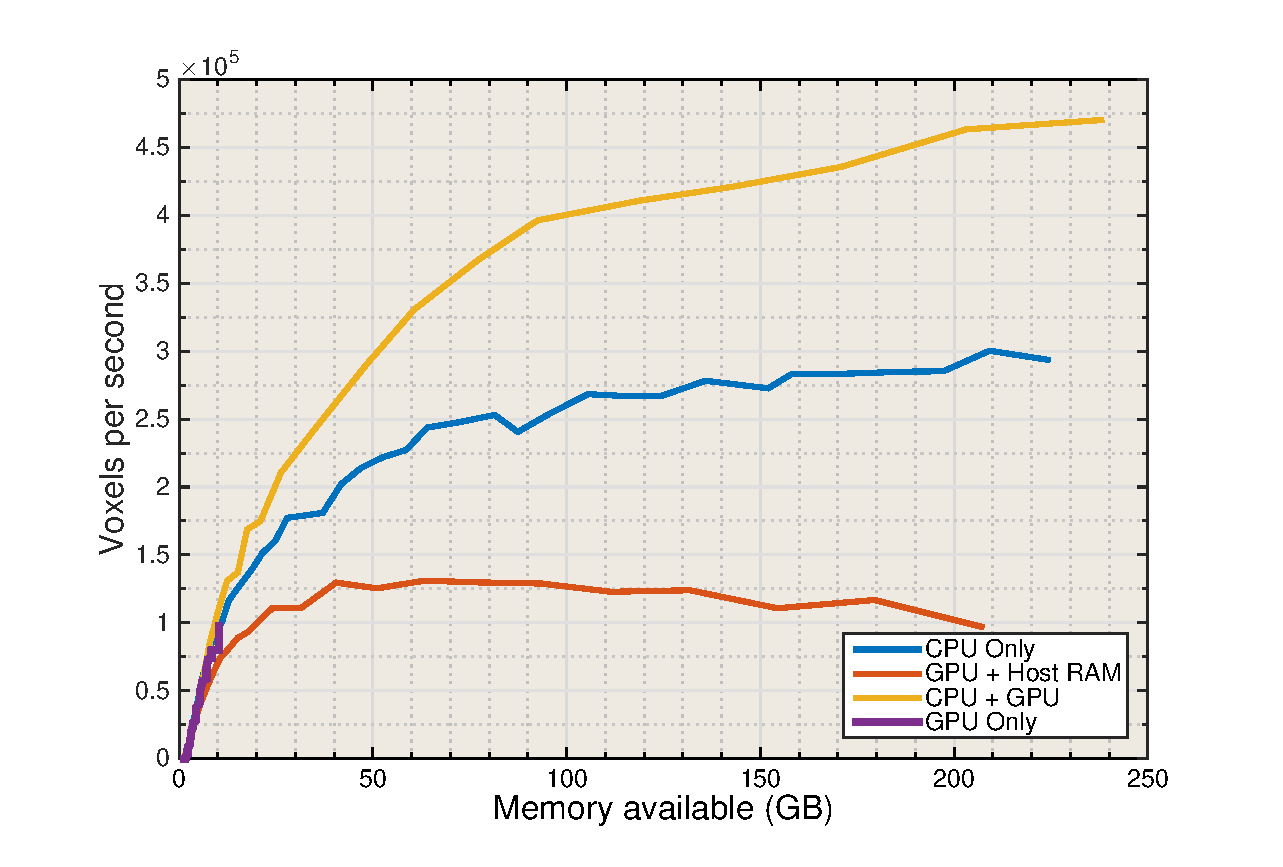
\includegraphics[trim= 10mm 2mm 15mm 5mm, clip, width=0.38\textwidth]
      {fig/m76x.eps}}
    \subfloat[]{\protect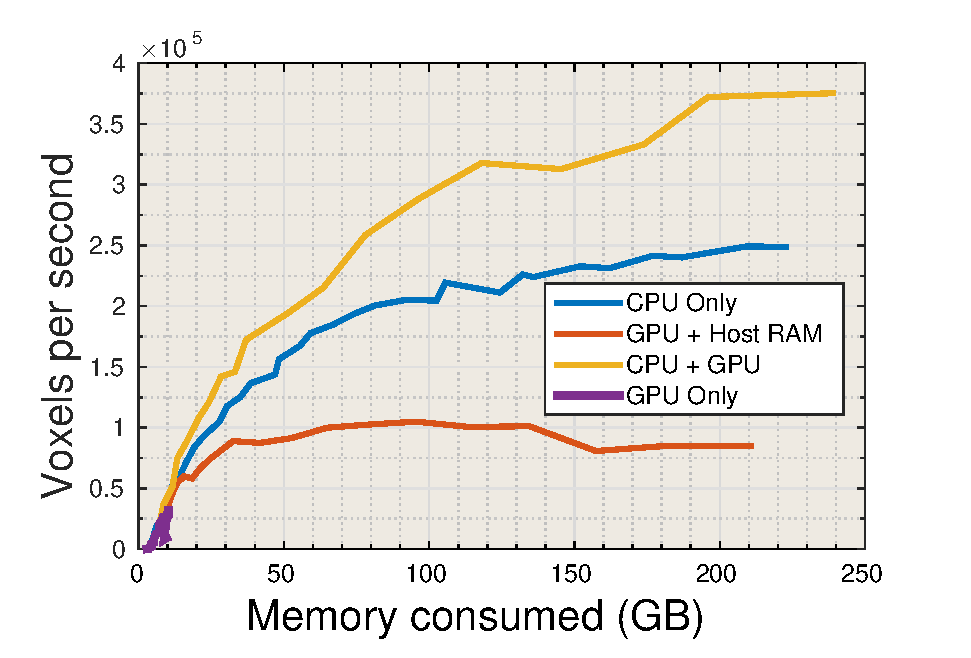
\includegraphics[trim= 10mm 2mm 15mm 5mm, clip, width=0.38\textwidth]
      {fig/m96x.eps}}

    \caption{Throughput vs memory available
    }
    \label{fig:final_results}
  \end{figure*}

  Our second set of benchmarks include more advanced network execution
  strategies.  We benchmark the four before--mentioned networks with
  the following four execution strategies.

  \subsubsection{CPU--only}

  The CPU--only network is performed layer at the time.  Task parallel
  FFT--based convolutional layers are used for all except the first
  layer, where data parallel FFT--based algorithm is used.

  \subsubsection{GPU + host RAM}

  First 4 layers are done layer at the time.  The convolutional layers
  ($1$st and $3$rd layer) are computed using the convolutional layer
  implementation that uses GPU for computation and host RAM for
  storage (cross reference).  The $2$nd and $4$th layers are computed
  using the CPU MFP implementation.

  As there are two pooling layers of size $2 \times 2 \times 2$ among
  the first four layers, the output of the fourth layer will have the
  first dimension of size $64$ (mini--batch size).  The rest of the
  network is then computed mini--batch at the time, where the size of
  minibatch is maximized so that it can fit on the GPU.

  \subsubsection{CPU + GPU}

  We divide the network into two parts.  The first part is processed
  by the CPU, layer at the time.  The second part is processed by the
  GPU -- minibatch at the time.

  This strategy allows for the CPU to start working on the next input
  while the GPU is processing the first input.  This forms a pipeline,
  but requires a bit more working memory.

  The optimal network division is empirically determined such that the
  computation time is evenly divided between the CPU and the GPU.  For
  {\tt n337} the CPU processes the first 4 layers, for {\tt n537} the
  CPU processes the first 6 layers, and for {\tt n726} and {\tt n926}
  the CPU processes the first 5 layers.

  \subsubsection{Optimized GPU-only}

  All computation is performed on the GPU, and all the data is stored
  on the GPU's RAM.  For given amount of available RAM we try to
  maximize the output image size.  Then, for each layer we empirically
  chose the fastest implementation.  It turns out that for the
  networks {\tt n337} and {\tt n537} it is optimal to use direct
  convolution (cuDNN with precomputed indices).  While for the
  networks {\tt n726} and {\tt n926} it is optimal to use FFT based
  convolutions for all except for the first layer, where it is better
  to use the direct convolution.

\section{Comparison to other algorithms}


  \begin{table*}[t]
    \centering
    \begin{tabular}{l|cccccccc}
      \toprule
      Network  & Baseline (cuDNN)    & Theano     & Caffe    & ELEKTRONN  & ZNN        & GPU-Only   & CPU-Only   & GPU-CPU \\
      \midrule
      n337     & $22934.8$           & $1979.3$   & $1.348$  & $122668$   & $34334.8$  & $666485$   & $262131$   & $933070$ \\
      n537     & $1048.68$           & --         & --       & --         & $9494.5$   & $28757.5$  & $194683$   & $334163$ \\
      n726     & $13520.4$           & $90.523$   & --       & $6122$     & $31354.8$  & $97413.4$  & $300312$   & $470166$ \\
      n926     & $2667.86$           & --         & --       & --         & $20908.6$  & $27667.8$  & $249190$   & $375295$ \\
      \bottomrule
    \end{tabular}
    \caption{Comparisons to other methods.}
    \label{table:conv_complexity}
  \end{table*}

  We implement the baseline algorithm ourselves, by simply calling
  cuDNN~\cite{chetlur2014cudnn} primitives.

  We compare our approach to Theano~\cite{bergstra2010theano} that
  computes sparse outputs, a version of Caffe~\cite{jia2014caffe} that
  is capable of producing dense output using strided
  kernels~\cite{tschopp2015efficient}, ELENTRONN~\cite{ELEKTRONN2015},
  and ZNN~\cite{zlateski2015znn}.

  The only package that has an optimization for inference is
  ELEKTRONN.

\section{Acknowledgments}
We are grateful to Intel Corporation for providing the 4–way Intel
Xeon E7–8890 v3 machine, and for support through an Intel Parallel
Computing Center.

%%%%%%%%%%%%%%%%%%%%%%%%%%%%%%%%%%%%%%%%%%%%%%%%%%%%%%%%%%%%%%%%%%%%%%%
%%%%%%%%%%%%%%%%%%%%%%%%%%%%%%%%%%%%%%%%%%%%%%%%%%%%%%%%%%%%%%%%%%%%%%%
%%
%% REFERENCES
%%
%%%%%%%%%%%%%%%%%%%%%%%%%%%%%%%%%%%%%%%%%%%%%%%%%%%%%%%%%%%%%%%%%%%%%%%
%%%%%%%%%%%%%%%%%%%%%%%%%%%%%%%%%%%%%%%%%%%%%%%%%%%%%%%%%%%%%%%%%%%%%%%

\clearpage

{\small
\bibliographystyle{IEEEtran}
\bibliography{IEEEabrv,./ref/bib}
}


\end{document}

%% r3.8xlarge
%% CUDNN GEMM not OK for 9x9x9
